\chapter{时间感知的标签推荐}
\label{chapter-wpitf}
本章重点介绍时间感知的标签推荐研究内容。首先,章节~\ref{sec-wpitf-intro}阐述标签推荐的研究背景、意义、研究贡献。其次,章节~\ref{sec-wpitf-related}讨论与标签推荐以及模型相关的研究工作。随后,章节~\ref{sec-wpitf-wpitf}重点介绍本章提出的标签推荐模型以及相关参数学习等。章节~\ref{sec-wpitf-exp}通过实验验证模型的有效性。最后总结本章标签推荐的研究内容。


\section{引言}
\label{sec-wpitf-intro}
分众分类标签系统如Delicious、Last.fm和豆瓣等互联网服务网站允许用户使用关键字标记书签、音乐、电影等资源(或者商品),这种行为被称为标注标签。标签是Web 2.0的一个重要的特征,它可以帮助用户管理自己收藏的资源,方便用户以一种简单的机制来协同管理或搜索网络中的资源(本章节中一般描述为商品)~\cite{dellschaft2012measuring}。图~\ref{fig-wpitf-douban}展示了豆瓣电影的标签系统。左图~\ref{fig-wpitf-doubana}展示了用户对电影显式反馈时利用标签对商品描述。用户对商品标注标签不仅标明了商品的属性,也说明了用户对商品的关注点,侧面反映了用户偏好。右图~\ref{fig-wpitf-doubanb}展示了用户通过标签来寻找自己感兴趣的电影,说明标签方便用户检索信息。

\begin{figure}
	\centering
	\subfigure[对电影标注标签]{
		\label{fig-wpitf-doubana}
		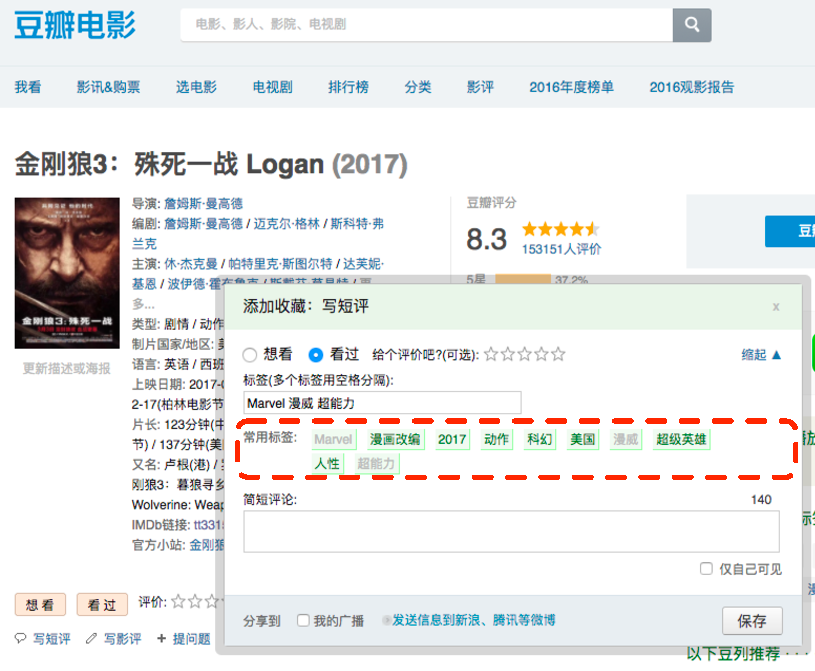
\includegraphics[width=0.45\textwidth]{Fig/wpitf/doubanTag}}
	\hspace{0.8cm}
	\subfigure[根据标签寻找电影]{
			\label{fig-wpitf-doubanb}
		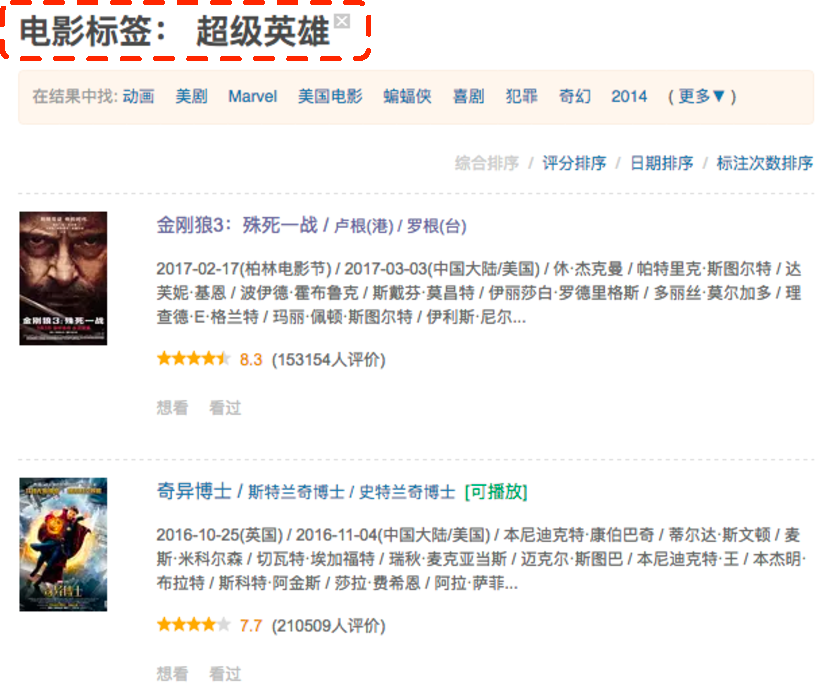
\includegraphics[width=0.45\textwidth]{Fig/wpitf/doubanTag1}}
	\caption{豆瓣电影标签例子}
	\label{fig-wpitf-douban}
\end{figure}

个人标签系统可以极大的提高网络商品的搜索效率~\cite{jaschke2008tag},同时可以准确刻画用户和商品的属性,帮助缓解冷启动问题\cite{lika2014facing},提高\textit{商品推荐}和\textit{评分预测}准确率~\cite{tso2008tag,zhen2009tagicofi,lacic2014recommending,saha2015predicting},促进推荐系统的良性循环。
但仍然有许多用户懒于给自己收藏的内容加上标签,因此需要个性化的标签推荐系统自动地给用户推荐标签,从而帮助用户更好地进行资源管理。目前的标签推荐方法分为两类:非个性化标签推荐方法和个性化标签推荐方法。非个性化的标签推荐系统针对某一资源,会给所有的用户推荐相同的标签,比如最流行标签模型,针对某一资源会给所有用户推荐目标资源上最热门的标签,这是一种非个性化的推荐。 而Rendle等人~\cite{rendle2009learning}已经验证了个性化推荐方法比理论上最优的非个性化的推荐方法的效果要好。个性化的标签推荐系统通过分析用户以往的标注标签行为来预测用户将会使用的标签,推荐结果由用户和商品属性共同决定。例如两个用户曾经对同一件商品标注过相同的标签,那么将来他们也有可能对另一商品使用相同的标签。也有可能一个用户近期大量使用某个标签,那么之后的一段时间也很可能还使用该标签对网络商品进行标记。进行个性化的推荐之所以有意义是因为对同样的资源,用户倾向于使用不同的标签,比如Last.fm提供非个性化的标签推荐,但用户仍然会使用不同的标签来标记音乐资源。

一些个性化标签推荐系统使用张量分解技术来为候选标签排序。基于张量分解的模型将用户-商品-标签张量分解成三个维度的特征矩阵,来表示与用户、商品、标签相关的隐含特征。基于Canonical分解的PITF\cite{rendle2010pairwise}张量分解方法,改进了基于Tucker分解的RTF\cite{rendle2009learning}模型复杂度与分解维度成立方比的缺点,使得模型运行时间与数据集的大小及特征维度均成线性关系,可以更好地处理高维分解,同时保持张量分解类算法较好的推荐新信息的能力,发现用户潜在的但自己尚未发现的兴趣偏好标签的优点。经典的张量分解类方法虽然有众多协同过滤的优点,但它们没有考虑到用户打标签的行为会随时间变化这一特征,以及较难处理好稀疏性、新用户冷启动等问题。因此最近出现了一些基于时间和频次的标签推荐系统BLL(Base-Level Learning)类方法,GIRP\cite{zhang2012integrating}, GIRPTM\cite{zhang2012integrating},BLL\cite{anderson2004integrated},BLLac\cite{kowald2015forgetting}等,这些方法仿照人脑存取长期记忆的方式,认为用户会倾向于再次使用自己最近最多使用过的标签。其中BLL类方法利用用户以往打标签行为与当前时间的间隔、标签的使用频次来估计用户将来重复使用某一标签的概率,并结合该网络商品中最流行标签进行推荐。但此类方法只能推荐历史记录中有的标签,没有推荐新标签的能力。

综合分析和考虑上述两类方法的优缺点,本章节提出时间感知的PITF模型(Time Aware PITF,简称TAPITF),在PITF模型的基础上增加对用户-标签-时间关系的权重以及商品-标签关系的权重,使得TAPITF模型既能考虑用户打标签行为和商品关注点随时间变化而变化的现象,也能有效地利用相似用户、相似商品、相似标签的信息,从而更好地对用户给商品标注标签的行为进行建模,提高标签推荐的准确度和新颖性。最后, 本章节在Movielens、LastFM和 Delicious三个数据集上进行了对比实验,实验结果表明本章节提出的方法在准确性上优于当前最新的标签推荐算法,同时还有较好的推荐新标签的能力。

\section{相关工作}
\label{sec-wpitf-related}
尽管在章节~\ref{chapter-related-coll}介绍了推荐系统中相关的协同过滤算法,但是它重点介绍\textit{商品推荐}和\textit{评分预测}两个任务。本小节将重点介绍个性化标签推荐的相关工作。

最简单的个性化标签推荐方法是用户最流行标签模型,给用户推荐用户自身使用最多的标签。Hotho等人~\cite{hotho2006information}提出自适应的PageRank(APR)算法,其主要思想是类似于网页的PageRank算法,即如果一个商品被重要的用户用重要的标签标注过,那么它也是个重要的商品。工作~\cite{marinho2008collaborative}使用了协同过滤思想,通过计算用户相互之间的相似度计算用户对某个商品标注标签的喜好值。Robert等人~\cite{jaschke2007tag}结合PageRank算法和用户之间的相似度,提出了FolkRank算法,使得推荐效果优于简单的基于频率的算法。张量分解模型也被广泛用于标签推荐。文章~\cite{symeonidis2008tag}使用了HOSVD模型~\cite{de2000multilinear},将三维的标签数据矩阵平铺成三个二维的矩阵,然后利用SVD算法建模用户、商品和标签隐藏特征。HOSVD模型需要对三个矩阵进行SVD分解,增加了模型训练时间,工作~\cite{rendle2009learning}提出了基于Tucker分解~\cite{tucker1966some}的张量分解模型RTF-TD,通过最大化AUC直接对标签数据进行三维分解。因为RTF-TD模型在预测标签推荐时间复杂度是隐藏特征向量维度的三次方,Rendle等人提出了PITF模型\cite{rendle2010pairwise},显式地对用户、商品、标签两两之间的关系进行建模,有效地利用相似用户、相似商品、相似标签等信息来进行标签推荐,并且将预测复杂度降为与隐藏特征向量维度成正比。NLTF~\cite{fang2015personalized},使用高斯径向基核函数以非线性方式扩展了张量分解模型,用来捕捉用户描述商品的复杂行为,期望更好地刻画用户、商品、标签的内在属性。除此之外,主题模型也被用来进行标签推荐,代表性方法有基于LDA主题模型的标签推荐系统\cite{krestel2009latent},该方法使用拥有大量标签的商品来抽取隐含的主题,然后把待标注的商品映射到相应的主题上,把属于这些主题的标签推荐给用户。

上述模型忽略了用户标注标签的行为会随时间变化这一现象\cite{yin2011temporal}。因此最近的研究工作尝试在进行标签推荐时考虑时间因素,Zhang等人\cite{zhang2012integrating}基于用户打标签行为的频次和时间提出了GIRP模型,对标签第一次被使用及最后一次被使用的时间对用户重复使用标签的概率建模。GIRPTM模型\cite{zhang2012integrating}扩展了GIRP模型,推荐时考虑了目标商品上最热门的标签,同时解决新用户冷启动问题。考虑时间的因素还有基于认知科学的BLL类模型,包括BLL$_{AC}$~\cite{kowald2015forgetting}、BLL+MP$_m$~\cite{kowald2014long}、BLL$_{AC}$+MP$_m$~\cite{kowald2015refining}、3LT+MP~\cite{kowald2015forgetting}~\cite{seitlinger2013recommending}。 BLL模型认为用户会倾向于再次使用自己最近最多使用过的标签,利用幂函数对这一行为启发式建模。BLL$_{AC}$~\cite{kowald2015forgetting}扩展了BLL,除了使用长尾分布对用户历史行为的频次和时间间隔进行建模外,还增加了关联模块(Association Component)描述目标资源的特征对用户的影响,即用户不一定总是选择自己最近最多使用过的标签,会随着目标资源的不同做出调整,但只会给用户推荐他之前使用过的标签。BLL+MP$_m$~\cite{kowald2014long}和BLL$_{AC}$+MP$_m$~\cite{kowald2015refining}分别扩展了BLL和BLL$_{AC}$,都考虑给用户推荐目标资源上最热门的标签。 3LT+MP模型~\cite{seitlinger2013recommending}除了利用用户对标签的遗忘规律,还使用LDA来模仿用户存取记忆时访问的语义场,以便更好地刻画用户画像和商品属性,提高推荐的准确度。

本章节工作中对时间信息的建模方法与BLL类模型相比主要区别是:BLL类方法利用幂函数叠加的方式计算用户每次使用标签的影响,当前时间改变后需要根据当前时间与用户每次访问该标签的时间重新计算喜好值,而本章节中从时间点过程(Temporal Point Process)对时间信息建模角度出发,利用指数函数将其从叠加转化为递归形式,使得计算当前时间下用户对标签的喜好值只跟上次使用标签的时间有关,极大地减少了计算时间。

%(2)标签是用户对商品的关注点描述,用户会随着时间的变化对商品的关注也不同,因此本章节工作认为商品被标注的标签也是随着时间的变化而变化,需要使用类似于建模用户标注标签的方法对该情况建模,而BLL类方法在对商品-标签建模时只是简单地统计全部数据中商品标签的频率信息,既没有考虑时间信息对商品标签的影响,同时包含目标用户在目标商品上标注目标标签的时间之后的其他用户在该商品上使用该标签次数信息也是不合理的。

%\section{模型基础知识}
%\label{sec-wpitf-basic}


%\subsection{BLL+MP$_i$模型}
%BLL+MP$_i$~\cite{kowald2014long}使用用户以往打标签行为的频次(Frequency)及历史打标签行为时间与当前时间的间隔(Recency)来建模,同时考虑了目标资源上最热门的标签对用户的影响。
%
%首先根据某个标签被目标用户使用的记录来计算标签的活跃程度BLA(Base-Level Activation):
%\begin{equation}
%BLA(t,u)=\ln (\sum_{i=1}^{n}(s_{ref}-s_{j})^{-d})
%\end{equation}
%其中$n$是标签$t$被用户$u$使用的总次数,第$j$次的时间戳 为$s_j$,$s_{ref}$表示用户当前要打标签的时间,时间间隔是两者的差值\footnote{ 原论文BLL代码: \url{https://github.com/learning-layers/TagRec/} 使用的是两者时间戳的差值$+1.0$,且时间戳以秒为单位。},d的取值为0.5\cite{anderson2004integrated}。经过归一化处理后:
%\begin{equation}
%||BLA(t,u)||=\frac{\exp (BLA(t,u))}{\sum_{t'=1}^{m}\exp (BLA(t',u))}
%\end{equation}
%其中$m$表示用户$u$使用过的标签的总数。
%
%除此之外该模型还考虑了用户当前所处上下文中的语义提示信息,即MP$_i$,表示的是目标资源$i$上最热门的标签。给定用户-资源对$(u,i)$,推荐标签预测分数可以下公式计算:
%\begin{equation}
%\hat{y}_{u,i,t}=\beta ||BLA(u,t)||+(1-\beta)|||Y_{t,i}|||
%\end{equation}
%$\beta$为调节用户-标签和资源-标签偏好的权重,当$\beta=0.0$时模型退化为MP$_i$模型,当$\beta=1.0$时模型变为基本的BLL模型,$|Y_{t,i}|$表示目标资源$i$在标签$t$上的数量。


\section{时间感知的逐对排序张量分解模型}
\label{sec-wpitf-wpitf}
本章节主要介绍时间感知的标签推荐模型。本小节首先介绍利用时间点过程中的Hawkes过程对用户给商品标注标签的时间信息建模。因为原始Hawkes过程是一个累加过程,需要随着时间推移需要重新计算,本章工作针对这一缺点将其改进成一个递归形式,降低预测标签喜好值的计算时间复杂度。然后,本章工作将时间建模信息以权重的方式与张量分解模型结合得到时间感知的PITF模型(Time Aware PITF,简称TAPITF)。章节中未介绍的符号说明详见章节~\ref{sec-c2-basic}中表~\ref{tab-basic-notation}。下面开始具体地介绍TAPITF模型。

\subsection{时间信息建模}
\label{sec-wpitf-time}
时间点过程~\cite{schoenberg2010introduction}是描述时序关系离散事件的随机过程。例如用户标注标签中,每个点表示用户在某一时刻标注标签,每个点以时间顺序排列,通过点之间的时间间隔描述整个点过程。本章节工作利用时间点过程中\textbf{Hawkes过程}~\cite{hawkes1971spectra}对标签时间信息建模。Hawkes过程是泊松过程的非马尔科夫扩展,表现一种``自我激励''的过程,每次事件的发生影响未来时间段事件的重新发生。Hawkes过程的条件强度定义如下:

\begin{equation}
\label{equ-wpitf-hawkes}
\tau(s) = \tau_0 + \sum_{s_i<s}E(s,s_i)
\end{equation}
其中$E(s,s_i)\geq 0$是用来描述时间间隔的激励函数,$\tau_0$是初始强度。用户一般会在连续一段时间内访问某类相似商品,会使用相同的标签描述商品特性。另外,因为用户的个人语言习惯,有多个词表示同一个意思(例如``风景''和``景色")时,用户偏向使用自己熟悉的词。因此,用户偏向使用近期较多使用的标签,符合上述``自我激励''的Hawkes过程。本章节工作利用上述Hawkes过程的条件强度来拟合用户使用标签的行为。

\begin{figure}
	\centering
	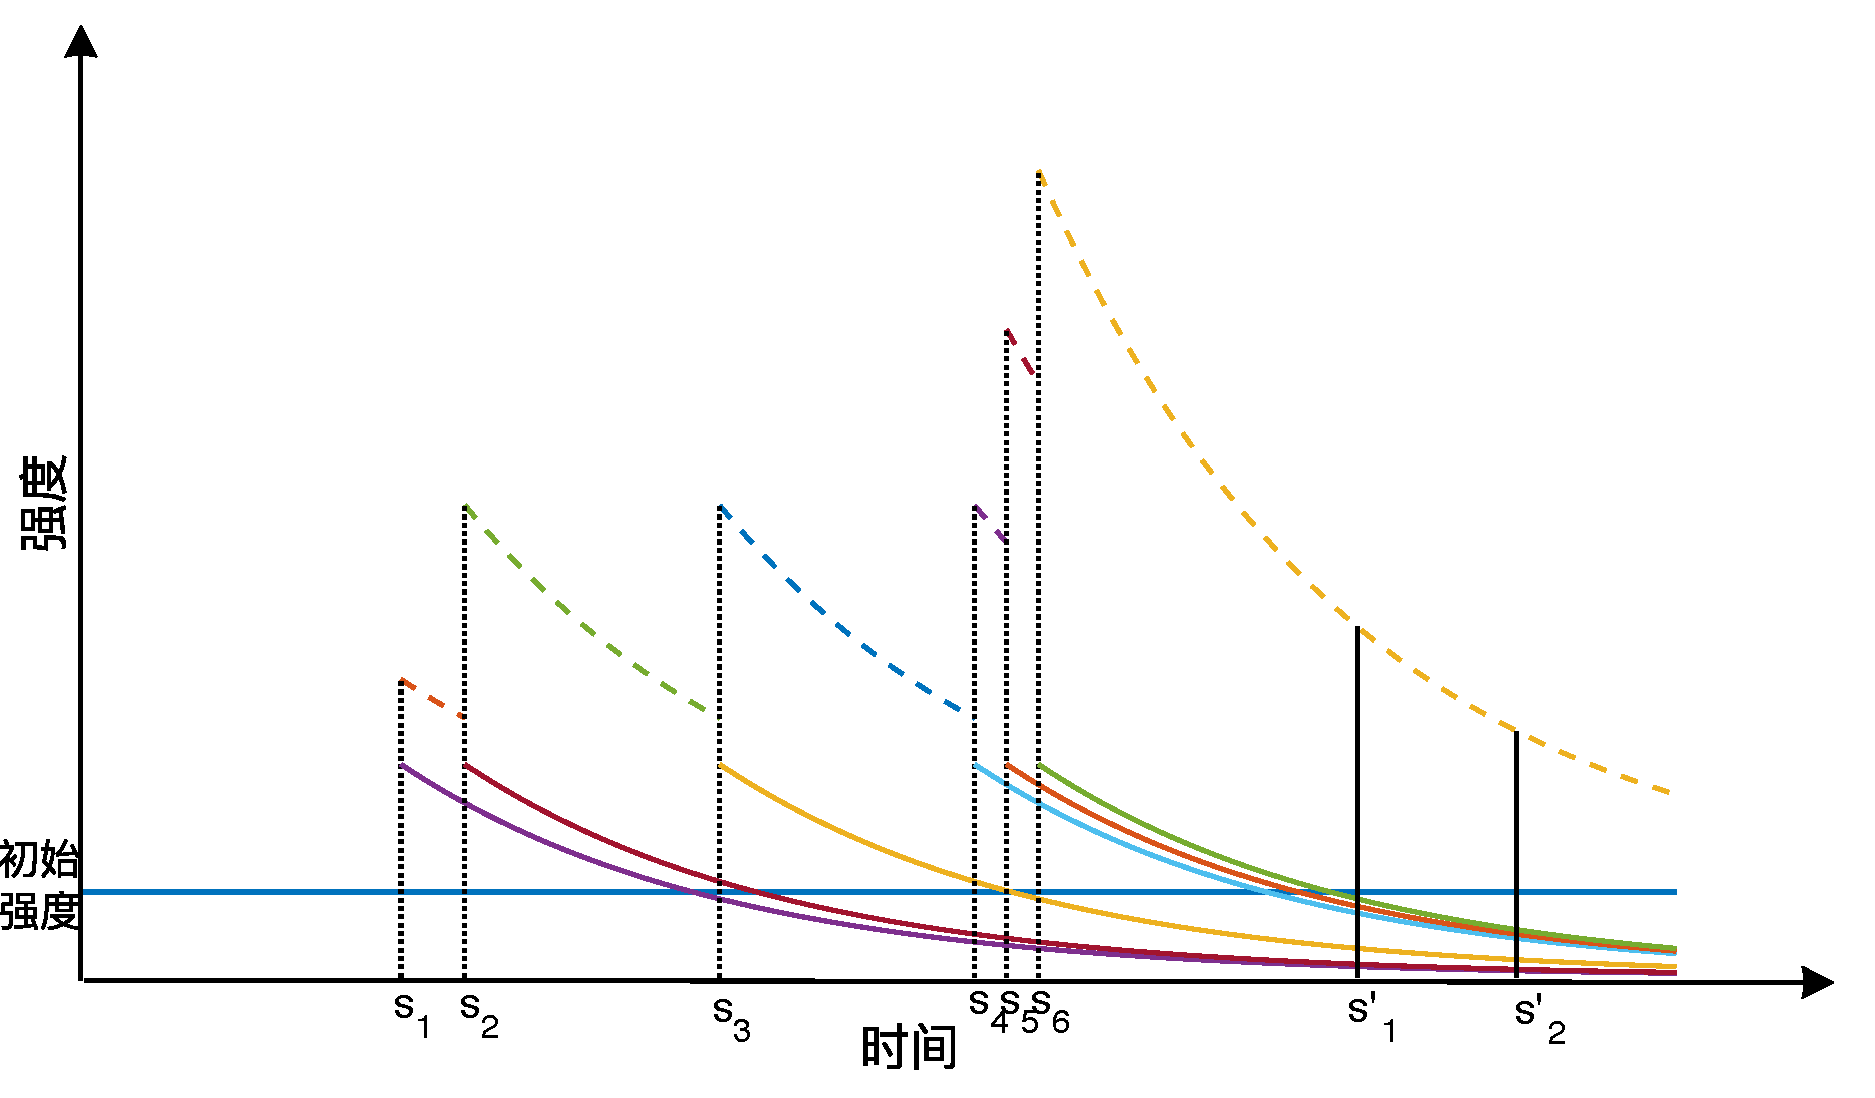
\includegraphics[width=0.9\textwidth]{Fig/wpitf/tagHawkes}
	\caption{Hawkes过程的条件强度函数示例}
	\label{fig-wpitf-tagHawkes}
\end{figure}

如果$\tau_0=0$以及激励函数设置为幂函数$E(s,s_i)=(s-s_i)^{-d}$,其中$d$是强度参数,那么这个函数等同于BLL类论文~\cite{kowald2014long,kowald2015forgetting,kowald2015refining}中对时间建模的函数。本章节工作中激励函数不同于上述设置,而是使用了指数函数$E(s,s_i)=\exp^{-d(s-s_i)}$。本章节工作使用指数函数作为激励函数一方面是因为幂函数和指数函数对最终标签推荐性能相差不大,另一方面主要是指数函数通过变化可以将叠加形式转换为递归形式,极大降低算法复杂度,特别是后面小节与PITF模型结合后参数学习的复杂度。图~\ref{fig-wpitf-tagHawkes}展示了激励函数为指数函数的Hawkes过程条件强度函数示例,其中$s_1, s_2,..., s_6$是事件发生的时间戳,彩色实线是每次事件发生后对未来事件的影响值,彩色虚线表示所有过去事件对未来事件的影响,任务是计算在$s'_1$和$s'_2$时刻的强度值。可以发现,每次事件发生都会增加未来时间发生率,并且随着时间的增加,影响越来越少。根据公式~\ref{equ-wpitf-hawkes},得到$s'_1$时刻的强度值需要计算并求和之前6次事件发生时间到$s'_1$的激励值,之后计算$s'_2$时刻的强度值又需要重新计算6次。也就是说每次计算某一时刻某个时间可能发生的强度值,都需要计算该时刻之前发生的所有事件对现在的影响。而指数函数作为激励函数,可以将加和形式转化为递归形式,还是图~\ref{fig-wpitf-tagHawkes}的例子,计算$s'_1$时刻激励函数之和$\tau^*(s'_1)$如下转化:

\begin{align}
\tau^*(s'_1) &= \sum_{i=1}^6E(s'_1,s_i)=\sum_{i=1}^6 \exp^{-d(s'_1-s_i)}\nonumber\\
&=\exp^{-d(s'_1-s_6)}\big(1+ \sum_{i=1}^5\exp^{-d(s_6-s_i)}\big)\nonumber\\
&=\exp^{-d(s'_1-s_6)}\big(1+\tau^*(s_6)\big)
\end{align}
可以发现是$s'_1$时刻事件发生的强度值只跟前一个事件发生$s_6$时刻的强度值有关。该现象说明只要预先计算完成所有事件发生时刻的强度值,任意时刻$s$的强度值只需要根据在$s$之前离$s$最近的事件发生时的强度即可求得。具体地,第$u$个用户在时刻$s$使用第$t$个标签的强度为:
\begin{equation}
\label{equ-wpitf-hawkes-user}
\tau(u,t,s) = \sum_{s_i<s} \exp^{-d(s-s_i)}= \exp^{-d(s-s_{last})}\big(1+\tau(s_{last})\big)
\end{equation}
其中$\tau_0=0$,$s_{last}$指的是离$s$最近的事件发生的时间。

\subsection{模型构建与学习}
从BLL类论文中可以发现利用用户打标签的时间戳信息建模,模拟用户倾向于再次使用自己最近最多使用过的标签的行为,同时考虑了目标资源最热门的标签,解决新用户冷启动问题,在标签推荐情境下能有较高的准确率。然而此类方法只能够推荐用户本来就熟悉的标签或者是目标商品最热门的标签,完全没有推荐新标签的能力。而张量分解模型是协同过滤的推荐方法,具有协同过滤方法的优点,譬如有推荐新信息的能力,发现用户潜在的但自己尚未发现的兴趣偏好标签等。然而此类模型缺少了时间和内容信息,没有对用户标签记忆模式建模,以及在冷启动情况下推荐效果不佳。

因此,本文综合考虑上述两类模型的优缺点,提出时间感知的的逐对张量分解模型(Time Aware PITF,简称TAPITF),其对用户-商品$<u,m>$的预测值如下:

\begin{equation}
\label{eq-wpitf-prediction}
\hat{y}_{umt}^s=w_{ut}^{s}\mathbf{P}_u^\top\mathbf{T}_t^{\mathcal{P}}+w_{mt}\mathbf{Q}_m^\top\mathbf{T}_t^{\mathcal{Q}}
\end{equation}
其中$w_{u,t}^s$是用户-标签-时间$<u,t,s>$权重,$w_{i,t}$是商品-标签对$<m,t>$权重。当第$u$个用户在时间$s$之前标注第$t$个标签的次数越多,且时间越近,那么用户-标签-时间$<u,t,s>$权重$w_{ut}^s$越大。类似地,所有用户在第$m$个商品标注第$t$个标签$t$的次数越多,那么商品-标签对$<m,t>$权重越大。同时需要保证当第$u$个用户在时间$s$前未标注过第$t$个标签时(或者没有用户在第$m$个商品上标注过第$t$个标签),权重$w_{ut}^s$和$w_{mt}$大于零以保证在历史记录中未出现过但相关的标签也能有机会被推荐给目标用户和目标商品。因此,针对权重$w_{ut}^s$,利用上一小节对时间建模信息的公式~\ref{equ-wpitf-hawkes-user}:

\begin{equation}
\label{eq-weight-uts1}
w_{ut}^s =1 + \log_{10}(1+10^{a^\mathcal{P}}\cdot ||\tau(u,t,s)||)
\end{equation}	
其中常数$\alpha^\mathcal{P}$是控制权重的增长速率。$||\tau(u,t,s)||$表示经过归一化的数值$||\tau(u,t,s)|| = \frac{\tau(u,t,s)}{\sum_{t\in \mathcal{T}_u}\tau(u,t,s)}$,$\mathcal{T}_u$表示第$u$个用户使用过的标签集合。当$||\tau(u,t,s)||$越大时,$w_{ut}^s$越大,且$||\tau(u,t,s)||=0$时,$w_{ut}^s=1$,也就是说第$u$个用户在时间$s$前未标注过第$t$个标签时,权重都为1。而针对权重$w_{mt}$,类似于BLL+MP$_m$~\cite{kowald2014long},本章工作利用商品最流行标签建立相应权重:


\begin{equation}
\label{eq-weight-it} w_{mt} = 1+\log_{10}(1+10^{a^\mathcal{Q}}\cdot \||\hat{\mathbf{Y}}_{mt}|\|)
\end{equation}
其中常数$\alpha^\mathcal{Q}$是控制权重的增长速率,$|\hat{\mathbf{Y}}_{mt}|$代表第$m$商品被第$t$个标签标记的次数。另外目标函数 Eq.~\ref{eq-wpitf-prediction}中$\mathbf{P}_u^\top\mathbf{T}_t^{\mathcal{P}}$(或者$\mathbf{Q}_m^\top\mathbf{T}_t^{\mathcal{Q}}$)继承了PITF的方法,能够较好地刻画用户、商品、标签三者的潜在向量特征,能够发现用户喜好(或者商品相关)但未发现的标签,提高推荐的新颖性。

 \begin{algorithm}
	\renewcommand\baselinestretch{1.3}\selectfont 	
	\begin{algorithmic}[1]
		\caption{TAPITF优化算法}
		\label{algo-tfwpitf-opt}
		\REQUIRE{用户对商品打标签历史记录$\{<u,m,t,s>\}$,隐藏向量维度$K$,学习速率$\iota$,正则化参数$\lambda$;}
		\ENSURE{用户隐藏特征向量$\mathbf{P}\in \mathbb{R}^{N \times K}$,商品隐藏特征向量$\mathbf{Q}\in \mathbb{R}^{M\times K}$,以及对应的标签隐藏特征向量$\mathbf{T}^\mathcal{P}\in \mathbb{R}^{T\times K}, \mathbf{T}^\mathcal{Q}\in \mathbb{R}^{T\times K}$;}
		
		\STATE {统计时间,频次,计算每条历史记录$y=<u,m,t,s>$的用户-标签-时间权重$w_{ut}^s$以及商品-标签权重$w_{mt}$;}
		\STATE {使用高斯分布$N(0,0.01)$初始化$\mathbf{P}, \mathbf{Q}, \mathbf{T}^\mathcal{P}, \mathbf{T}^\mathcal{Q}$;}
		
		\REPEAT 
		\STATE {从训练集中均匀采样$y=<u,m,t_A,s_A>$和对应的负样本标签$t_B$;}
		\STATE {根据$<u,t,t_B,s_A>$计算负样本的用户-标签权重$w_{ut_B}^{s_A}$;}
		\STATE {$\hat{y}_{umt_At_B}\leftarrow \hat{y}_{umt_A}-\hat{y}_{umt_B}$}
		\STATE {$\delta \leftarrow (1 - \sigma(\hat{y}_{umt_At_B}))$}
		
		\FOR{ $k$ from $1$ to $K$} 
		
		\STATE {$\mathbf{P}_{uk}\leftarrow \mathbf{P}_{uk}+\iota\cdot (\delta \cdot (\hat{w}_{ut_A}^{s_A}\cdot \mathbf{T}^\mathcal{P}_{t_Ak}-\hat{w}_{ut_B}^{s_A}\cdot \mathbf{T}^\mathcal{Q}_{t_Bk})-\lambda \cdot \mathbf{P}_{uk})$} 
		
		\STATE {$\mathbf{Q}_{mk}\leftarrow \mathbf{Q}_{mk}+\iota \cdot (\delta \cdot(\hat{w}_{ut_A}^{s_A}\cdot \mathbf{T}^\mathcal{P}_{t_Ak}-\hat{w}_{ut_B}^{s_A}\cdot \mathbf{T}^\mathcal{Q}_{t_Bk})-\lambda \cdot \mathbf{Q}_{mk})$}
		
		\STATE {$\mathbf{T}^\mathcal{P}_{t_Ak}\leftarrow \mathbf{T}^\mathcal{P}_{t_Ak}+\iota \cdot (\delta \cdot \mathbf{P}_{uk}\cdot w_{ut_A}^{s_A}-\lambda \cdot \mathbf{T}^\mathcal{P}_{t_Ak})$}
		
		\STATE {$\mathbf{T}^\mathcal{P}_{t_Bk}\leftarrow \mathbf{T}^\mathcal{P}_{t_Bk}+\iota \cdot (\delta \cdot (-\mathbf{P}_{uk})\cdot w_{ut_B}^{s_A}-\lambda \cdot \mathbf{T}^\mathcal{P}_{t_Bk})$}
		
		\STATE {$\mathbf{T}^\mathcal{Q}_{t_Ak}\leftarrow \mathbf{T}^\mathcal{Q}_{t_Ak}+\iota \cdot (\delta \cdot \mathbf{Q}_{mk}\cdot w_{mt_A}-\lambda \cdot \mathbf{T}^\mathcal{Q}_{t_Ak})$}
		
		\STATE {$\mathbf{T}^\mathcal{Q}_{t_Bk}\leftarrow \mathbf{T}^\mathcal{Q}_{t_Bk}+\iota \cdot (\delta \cdot (-\mathbf{Q}_{mk})\cdot w_{mt_B}-\lambda \cdot \mathbf{T}^\mathcal{Q}_{t_Bk})$}
		\ENDFOR		
		\UNTIL{收敛}		
		
		\RETURN {$\mathbf{P}, \mathbf{Q}, \mathbf{T}^\mathcal{P}, \mathbf{T}^\mathcal{Q}$}	
	\end{algorithmic}
\end{algorithm}

TAPITF使用BPR框架进行最大化成对排序目标函数,采用负采样随机梯度下降算法进行迭代优化,具体如算法~\ref{algo-tfwpitf-opt}所示。首先,在循环迭代之前,根据训练集标注标签的时间和频次统计,计算每条历史记录$y=<u,i,t,s>$中的用户-标签-时间$<u,t,s>$权重$w_{ut}^s$以及所有商品-标签对$<m,t>$的权重$w_{mt}$(第1行)。然后使用高斯分布分别初始化用户、商品、标签隐藏特征向量$\mathbf{P}, \mathbf{Q}, \mathbf{T}^\mathcal{P}, \mathbf{T}^\mathcal{Q}$(第2行)。每次迭代中,需要正样本和相应的负样本标签采样。因为正样本用户-标签-时间$<u,t,s>$权重$w_{ut}^s$和所有商品-标签对$<m,t>$的权重$w_{mt}$预先计算好了,所以只需计算负样本标签的用户-标签-时间$<u,t_B, s_A>$权重$w_{u,t_{B}}^{s_A}$。最后根据随机梯度下降公式进行迭代优化潜在向量(第3-15行)。


\subsection{时间复杂度分析}
\label{subsec-wpitf-timeAnalysis}
因为每条历史记录$y=<u,m,t,s>$中的用户-标签-时间$<u,t,s>$权重$w_{ut}^s$以及所有商品-标签对$<m, t>$的权重$w_{mt}$在迭代优化之前已经预先计算好,所以每次迭代只要计算负样本标签的用户-标签-时间$<u,m,t_B,s_A>$权重$w_{ut_B}^S$。因此每次迭代,复杂度相对于PITF(PITF每次迭代的复杂度为$O(K)$)来说多了计算$w_{ut_B}^{s_A}$的时间, 而计算权重$w_{ut_B}^{s_A}$又跟负采样的标签有关。由公式E.q.~\ref{eq-weight-uts1}和负样本采样方法中可以看出,$w_{ut_B}^{s_A}$的计算跟第$u$个用户,标注第$t_A$个正样本标签的时间$s_A$,第$u$个用户之前打过的标签,负样本标签$t_B$这几个方面有关。所以每次计算负样本用户-标签-时间$<u,m,t_B,t_A>$权重分两种情况:(1)负样本标签$t_B$不在第$u$个用户打过的标签集合中$\mathcal{T}_u$出现过,那么不需要计算,权重$w_{ut_B}^{s_A}=1$;(2)如果负样本标签$t_B$在第$u$个用户打过的标签集合中$\mathcal{T}_u$出现过,那么根据章节~\ref{sec-wpitf-time}分析,只需要二分搜索找到时间$t_A$之前第$u$个用户最近使用标签$t_B$的时间和预先计算好的权重即可得到负样本权重$w_{ut_B}^{s_A}$,因此复杂度为$O(\log(n_{ut_B}))$,$n_{ut_B}$代表第$u$个用户使用第$t_B$个标签的次数。这里假设每个历史记录循环迭代一遍,那么每条记录迭代计算$w_{ut_B}^{s_A}$的复杂度期望跟标签被使用的平均次数相关。因此,在最坏的情况下,也就是每次负采样的标签都是用户所使用过的标签,每次采样迭代的时间复杂度为$O(K+\log(n_{ut_B}))$。可以看出,如果数据集比较稠密的情况下,TAPITF每次迭代的运行时间会比PITF高一些。考虑到真实世界网络海量数据的稀疏性,TAPITF每次迭代的运行时间对比于PITF的运行时间增加的时间是有限的,在可接受的范围之内。

\section{实验及分析}
\label{sec-wpitf-exp}
本小节将介绍实验中用到的数 据集、实验设置、度量指标、评估方法以及实验结果。

\subsection{实验设置}

\subsubsection{数据集}
本实验中采用了三种互联网上可免费获取的标签数据集: Movielens、LastFM、Delicious\footnote{\url{http://files.grouplens.org/datasets/hetrec2011}}。三个数据集来自不同的领域,其中 Movielens 是一个电影推荐系统网站,LastFM 是一个网络电台和音乐社区,Delicious 则是一个书签网站。三个数据集的统计信息如表\ref{tab-wpitf-datasets}所 示,其中$U$表示用户-商品对数目,$U/M$体现数据集的稀疏程度。core定义了对数据集的过滤程度。$p$-core 表示数据集中的用户、商品以及标签在所有用户-资 源对中都至少出现$p$次。实验中选取了no core(完整数据集)和 core 3 两种情况。


% Table generated by Excel2LaTeX from sheet '工作表1'
\begin{table}[H]
  \centering
  \caption{标签数据集Movielens,LastFM和Delicious的统计信息}
      	  \label{tab-wpitf-datasets}
    \begin{tabular}{|c||c|c|c|c|c|c|}
    \hline
    \multicolumn{1}{|l||}{ } & \multicolumn{1}{l|}{core } & \multicolumn{1}{l|}{$N$ } & \multicolumn{1}{l|}{$M $} & \multicolumn{1}{l|}{$T$ } & \multicolumn{1}{l|}{$U$ } & \multicolumn{1}{l|}{$U/M$} \bigstrut\\
    \hline
    \hline
    \multirow{2}[4]{*}{Movielens } & -     & 2,113 & 5,908 & 9,079 & 27,712 & 4.69 \bigstrut\\
\cline{2-7}          & 3     & 656   & 2,376 & 2,061 & 18,427 & 7.76 \bigstrut\\
    \hline
    \multirow{2}[4]{*}{LastFM } & -     & 1,892 & 12,523 & 9,749 & 71,064 & 5.68\bigstrut \\
\cline{2-7}          & 3     & 1,277 & 5,940 & 2,761 & 59,692 & 10.05 \bigstrut\\
    \hline
    \multirow{2}[4]{*}{Delicious } & -     & 1,867 & 69,223 & 40,897 & 104,799 & 1.51 \bigstrut\\
\cline{2-7}          & 3     & 1,458 & 5,074 & 4,233 & 20,543 & 4.05 \bigstrut\\
    \hline
    \end{tabular}%
\end{table}%


\subsubsection{参数设置}
为了评价本章节提出的标签推荐模型,实验采用“留一 法”将数据集切分为训练数据集和测试数据集。当用户打过标签的商品数唯一时,则默认将这个用户-商品对放入训练集中。

在参数设置上,BLL+MP$_m$与BLL$_{AC}$+MP$_m$与\cite{kowald2014long}设置一样,权重因子$\beta=0.5, d=0.5$,时间以秒为单位;PITF与\cite{rendle2010pairwise}中设置一样,隐含维度$K=64$,正则化因子$\lambda=0.00005$,学习速率为0.05。本章模型中$d=0.005$,时间以天为单位, 隐含维度和正则化因子与PITF设置一样。PITF和TAPITF迭代轮数均为100轮。

\subsubsection{度量标准}
为了模拟真实世界标签推荐的环境,实验从两个维度去评估算法的性能:
\begin{itemize}
	\item \textbf{准确度:}准确度是推荐系统离线评测指标中最重要的一个。常见的指标有精准率(Precision)、召回率 (Recall)以及 F1 值,公式如下:
	\begin{eqnarray}
	\label{eq-wpitf-precision}
	Prec(S_{test},n)&=&\arg_{(u,m)\in P_{S_{test}}}\frac{|Top(u,m,n)\bigcap \{t|(u,m,n)\in S_{test}\}|}{n}\\
	\label{eq-wpitf-recall}
	Rec(S_{test},n)&=&\arg_{(u,m)\in P_{S_{test}}}\frac{|Top(u,m,n)\bigcap \{t|(u,m,t)\in S_{test}\}|}{|\{t|(u,m,t)\in S_{test}\}|}\\
	\label{eq-wpitf-f1}
	F1(S_{test},n)&=&\frac{2 \cdot	Prec(S_{test},n)\cdot Rec(S_{test},n)}{	Prec(S_{test},n)+Rec(S_{test},n)}
	\end{eqnarray}
	如果没有特别说明,实验使用 F1@5 衡量准确度。
	\item \textbf{新颖性:} 实验使用\cite{belem2013exploiting}中的 AIP@10 来定义推荐的标签列表的新颖性。如果推荐的标签从没标注过目标商品,则认为这个推荐是新颖的,所以对于目标商品,如果推荐的标签的流行程度越低,则新颖性越高。
\end{itemize}

\subsubsection{对比方法}
\begin{itemize}
\item \textbf{MP$_{m}$}:方法对给定目标资源会推荐该商品下最受欢迎的标签。
\item \textbf{PITF}~\cite{rendle2010pairwise}:由 Rendle 和 Schmidt-Thieme 提出的一种改 进的张量分解模型,显式地为用户、商品以及标签之 间的两两相互作用建模。
\item \textbf{BLL+MP$_m$}~\cite{kowald2014long}:将 BLL 与 MP$_m$ 结合,BLL 部分利用用户以往标注标签行为与当前时间的间隔、标签的使用频次来估计用户将来重复使用某一标签的概率。
\item \textbf{BLL$_{AC}$+MP$_m$}~\cite{kowald2015refining}:与 \textbf{BLL+MP$_m$} 类似,但是在 BLL 上 加入关联模块,描述目标商品的特征对用户的影响。 根据\cite{kowald2015evaluating}中标签推荐标准测试,该方法是当前准确度最好的标签推荐方法。
\end{itemize}

\subsection{实验结果及分析}
实验首先研究权重因子$\alpha$对 TAPITF 准确度的 影响,然后详细的对比 TAPITF 与其他标签推荐方法 的性能差异,最后从迭代的收敛速度以及算法运行时 间上对比 TAPITF 与 PITF 的差异。

\begin{figure}
	\centering
	\subfigure[Movielens (no core)]{
		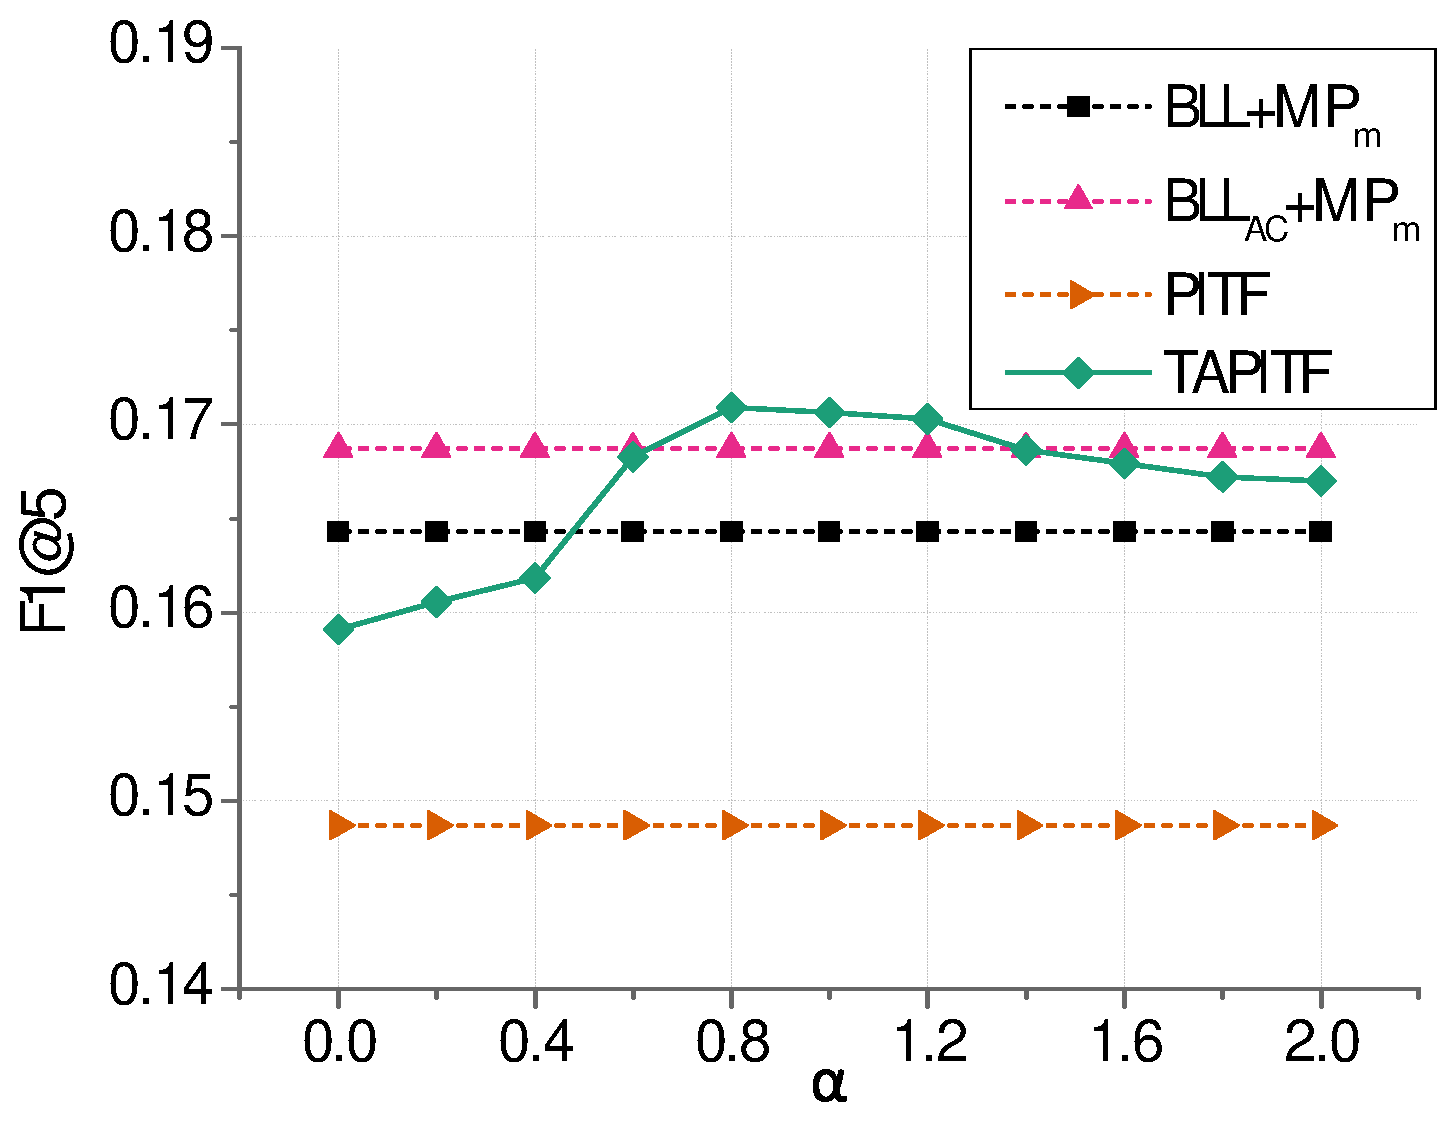
\includegraphics[width=0.485\textwidth]{Fig/wpitf/alpham1}}
	\hspace{0.0cm}
	\subfigure[Movielens (core 3)]{
		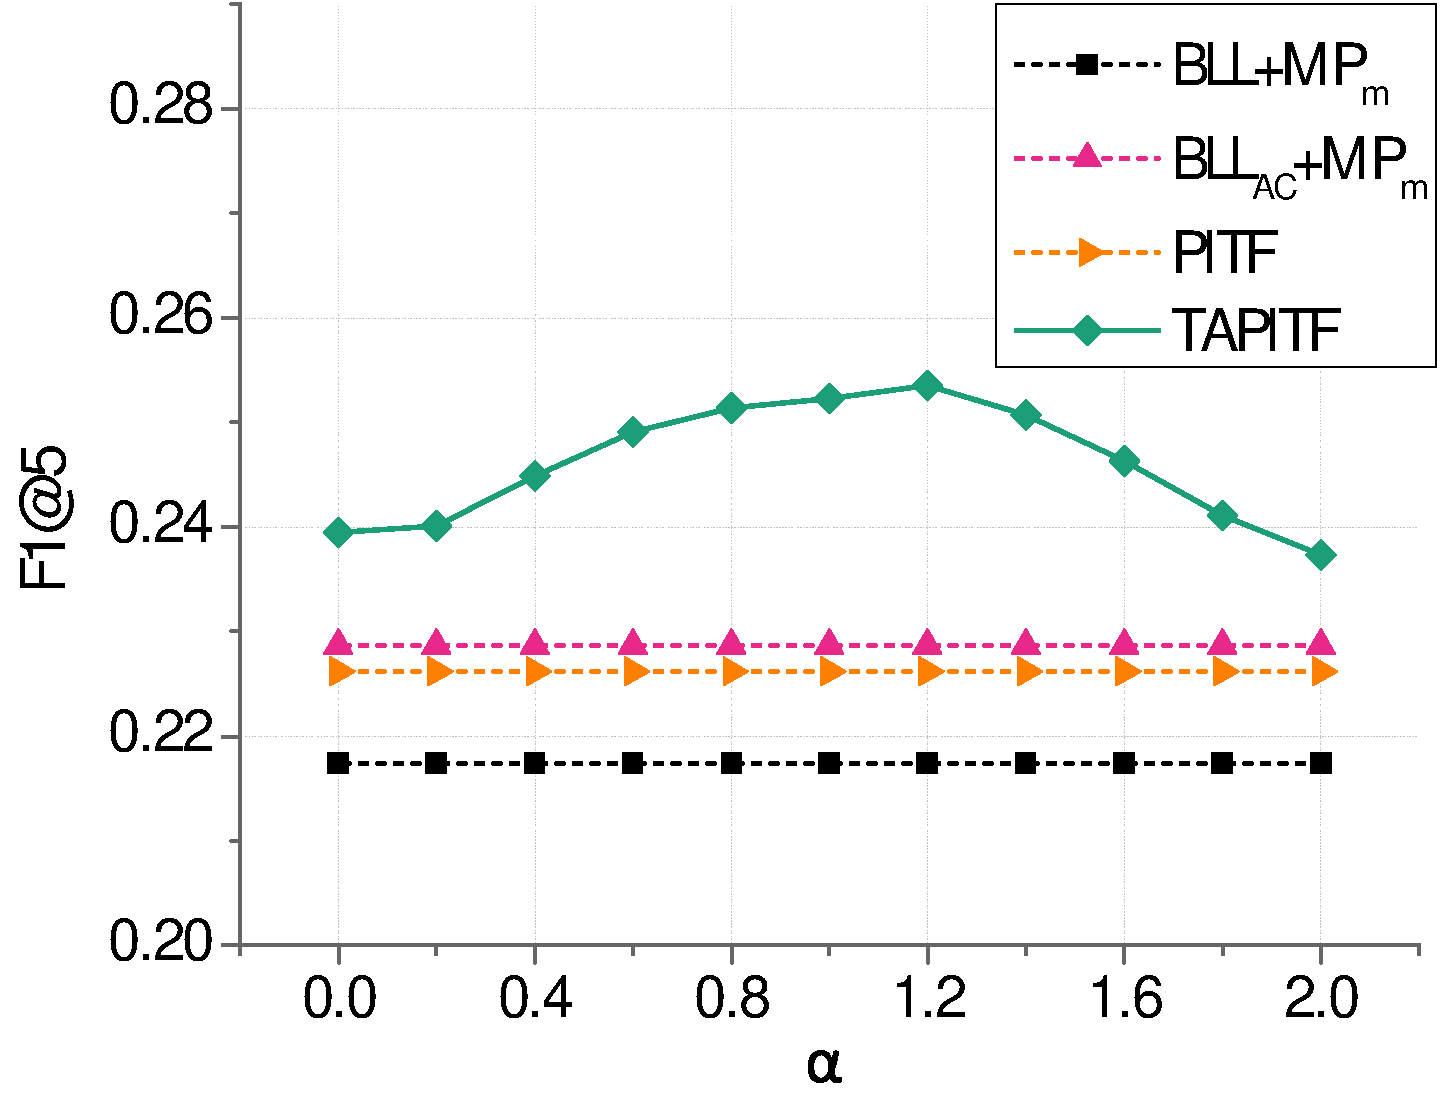
\includegraphics[width=0.485\textwidth]{Fig/wpitf/alpham3}}
	\subfigure[LastFM (no core)]{
		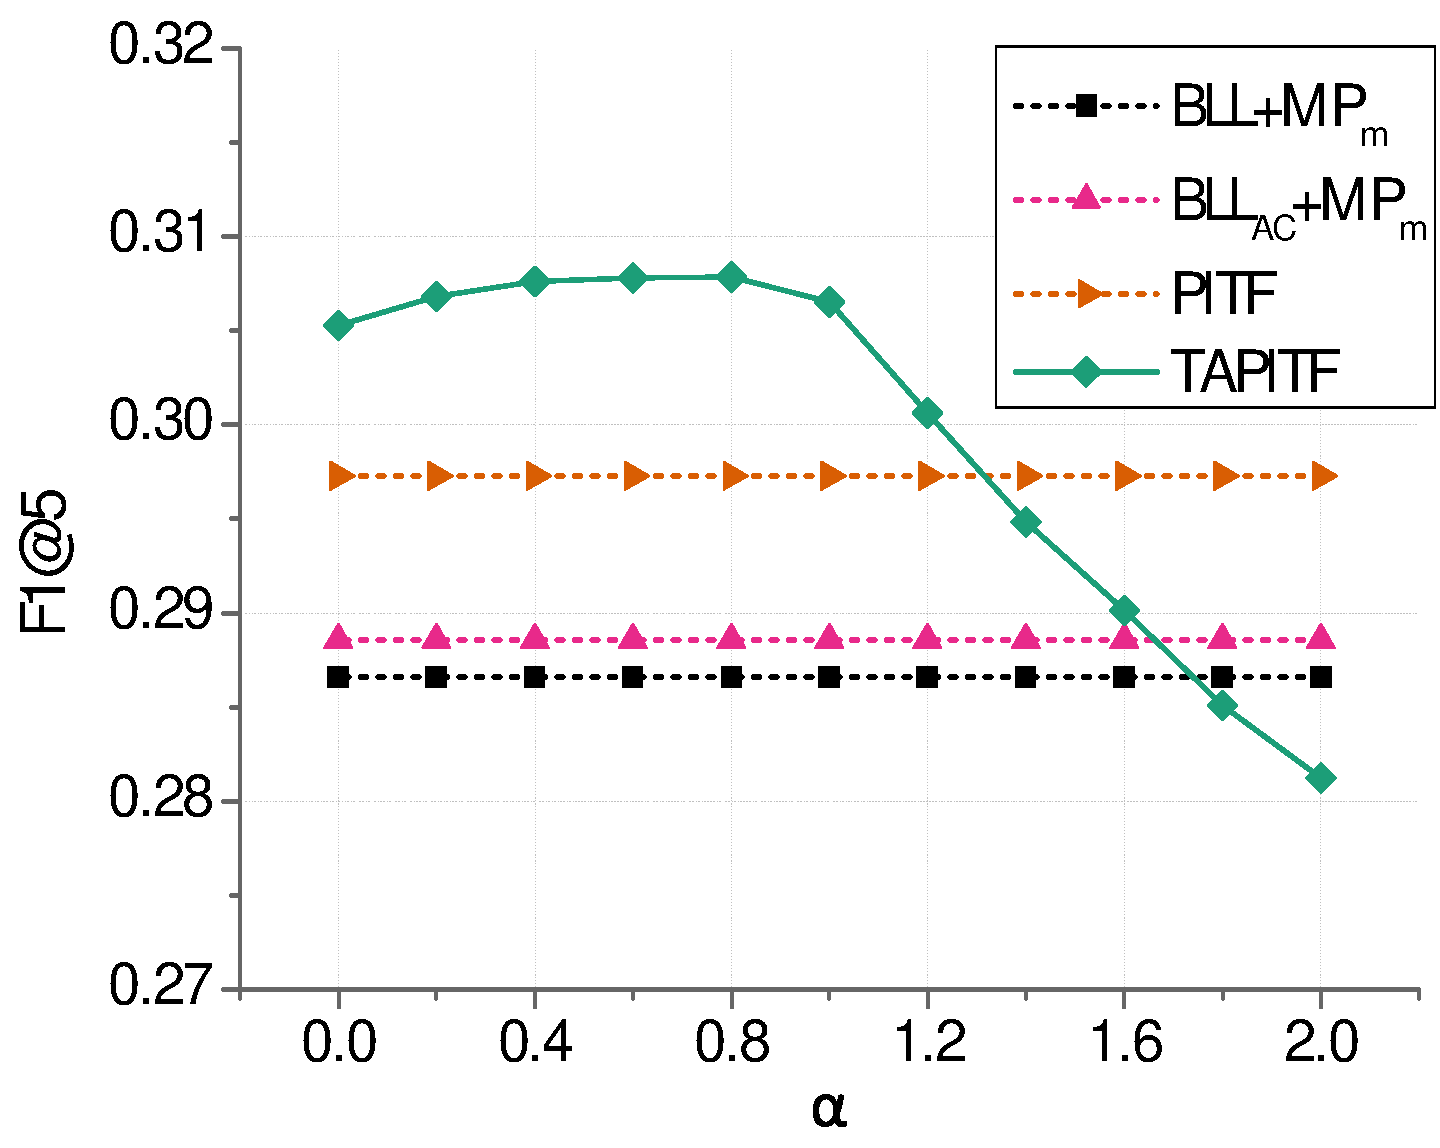
\includegraphics[width=0.485\textwidth]{Fig/wpitf/alphal1}}
	\hspace{0.0cm}
	\subfigure[LastFM (core 3)]{
		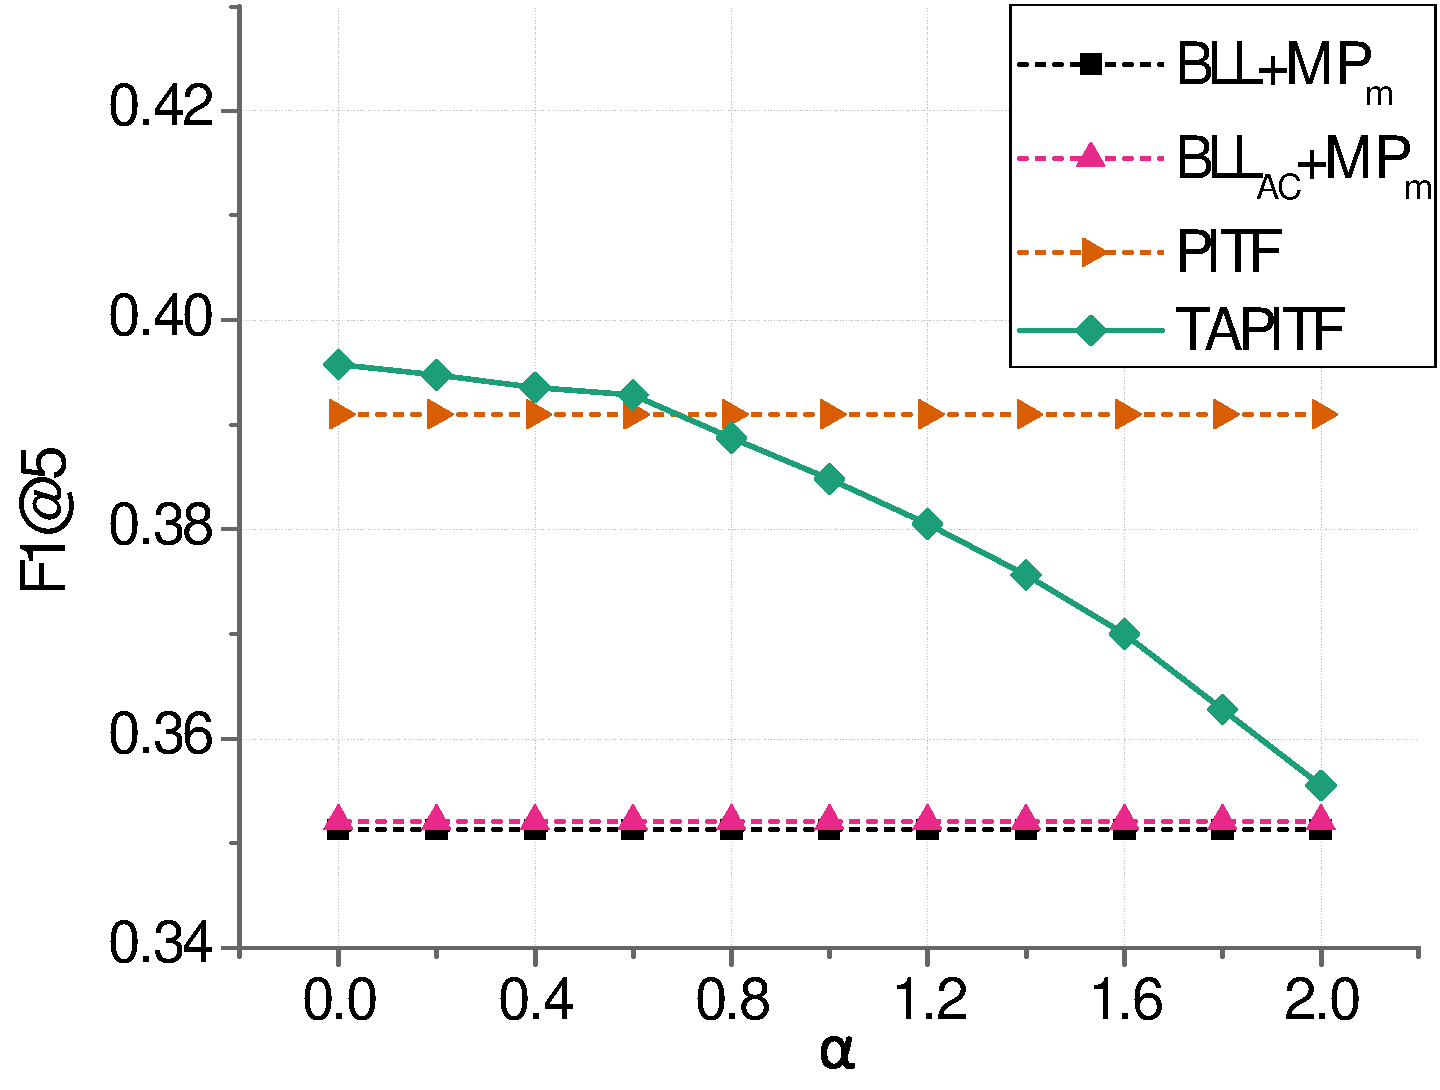
\includegraphics[width=0.485\textwidth]{Fig/wpitf/alphal3}}
	\subfigure[Delicious (no core)]{
		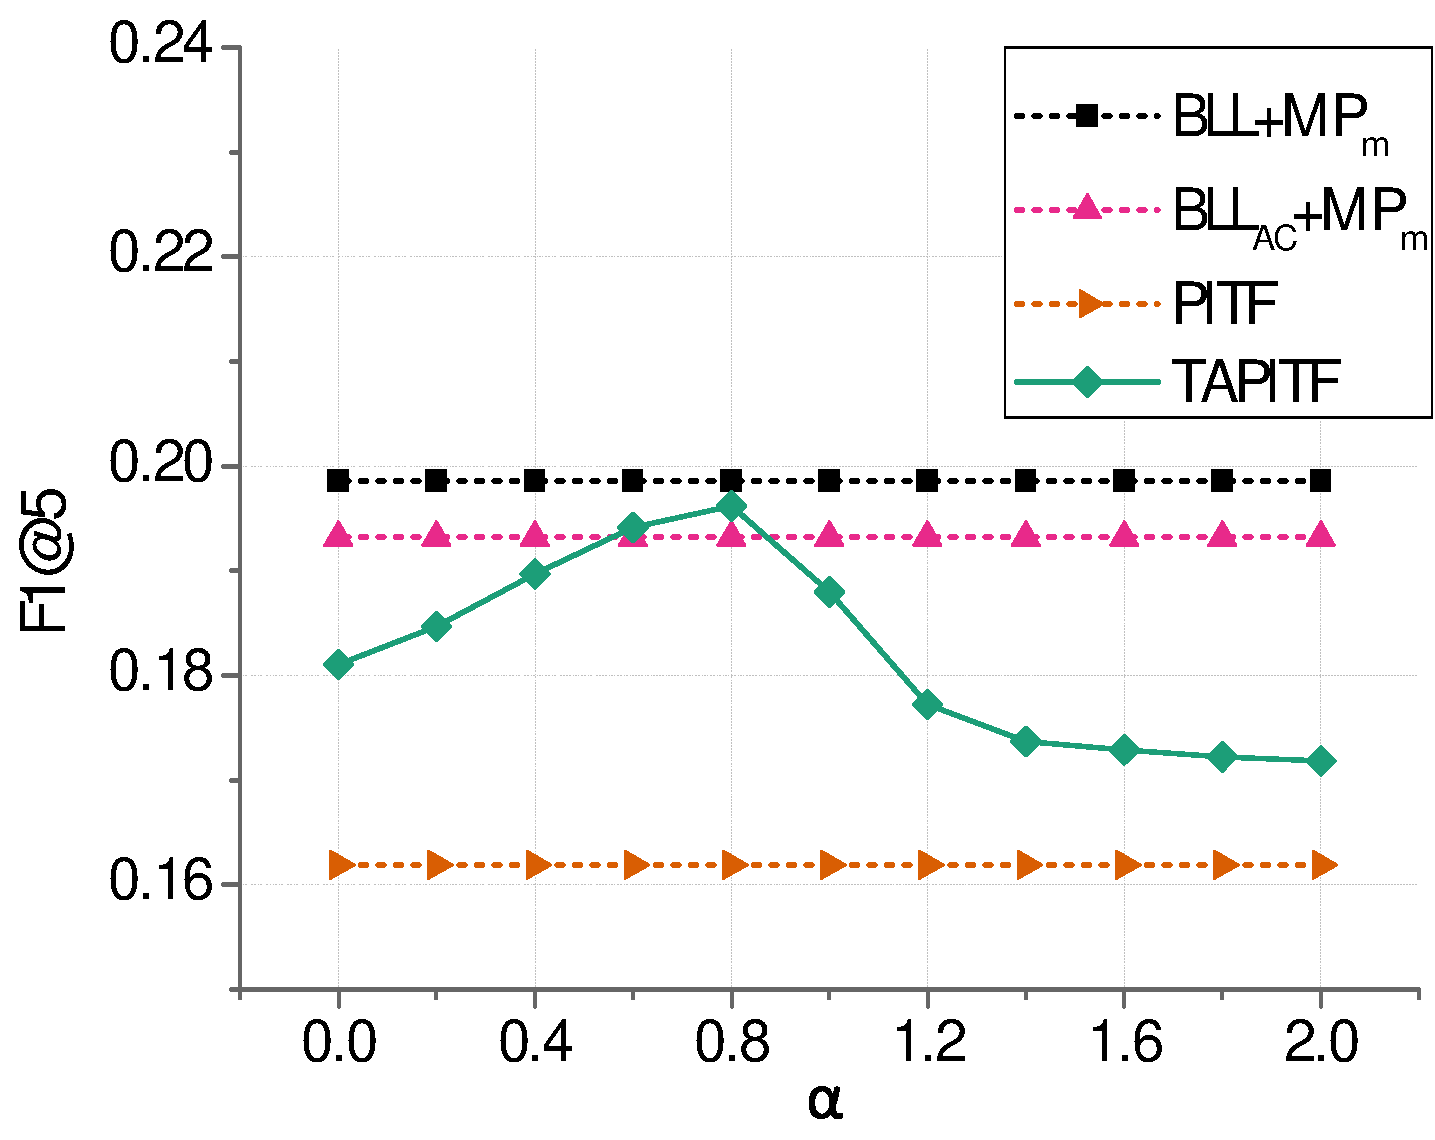
\includegraphics[width=0.485\textwidth]{Fig/wpitf/alphad1}}
	\hspace{0.0cm}
	\subfigure[Delicious (core 3)]{
		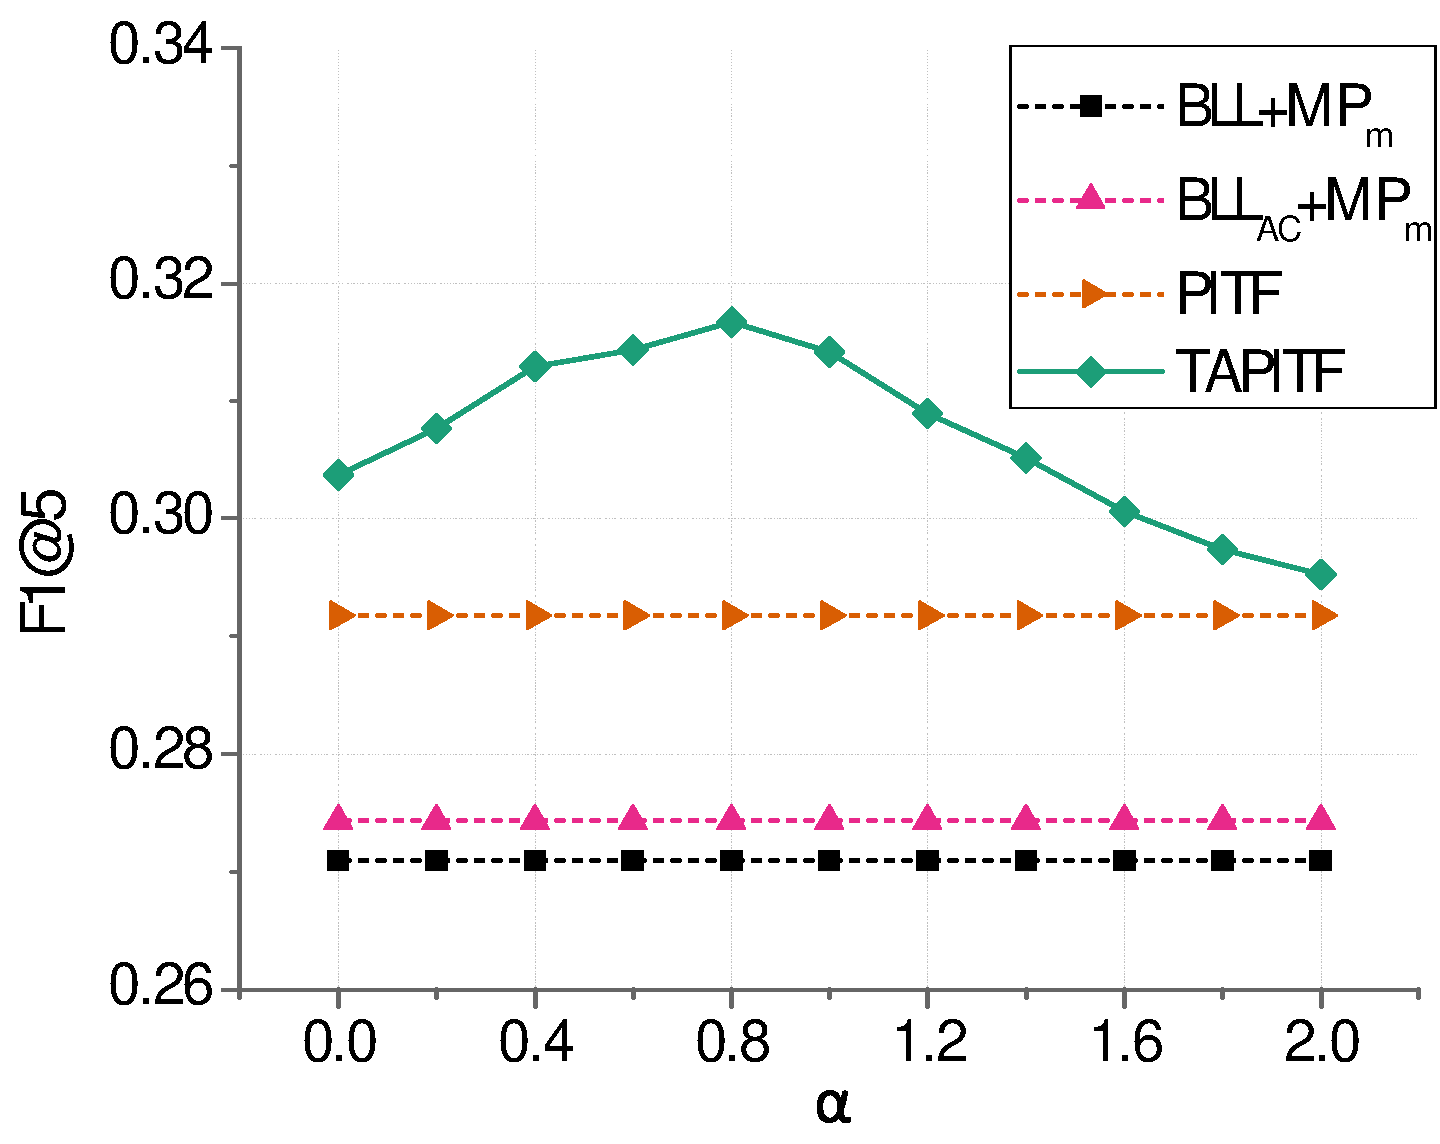
\includegraphics[width=0.485\textwidth]{Fig/wpitf/alphad3}}
    \caption{不同$\alpha$对推荐效果的影响}
	\label{fig-wpitf-alpha}
\end{figure}

\begin{figure}
	\centering
	\subfigure[Movielens (no core)]{
		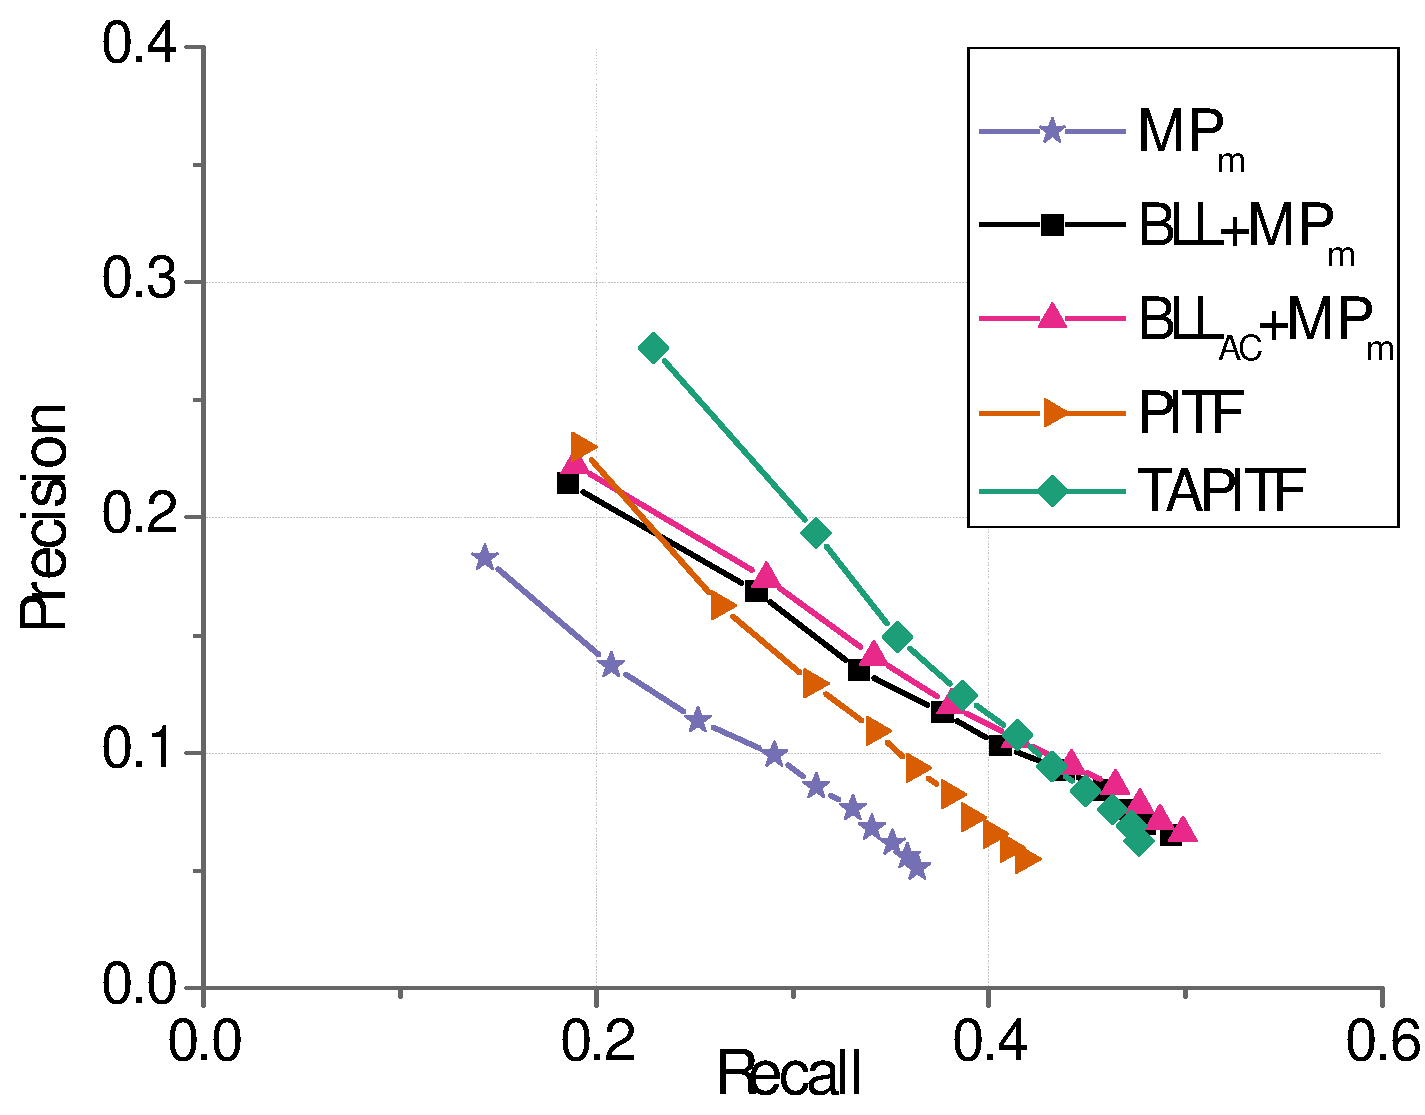
\includegraphics[width=0.485\textwidth]{Fig/wpitf/prm1}}
	\hspace{0.0cm}
	\subfigure[Movielens (core 3)]{
		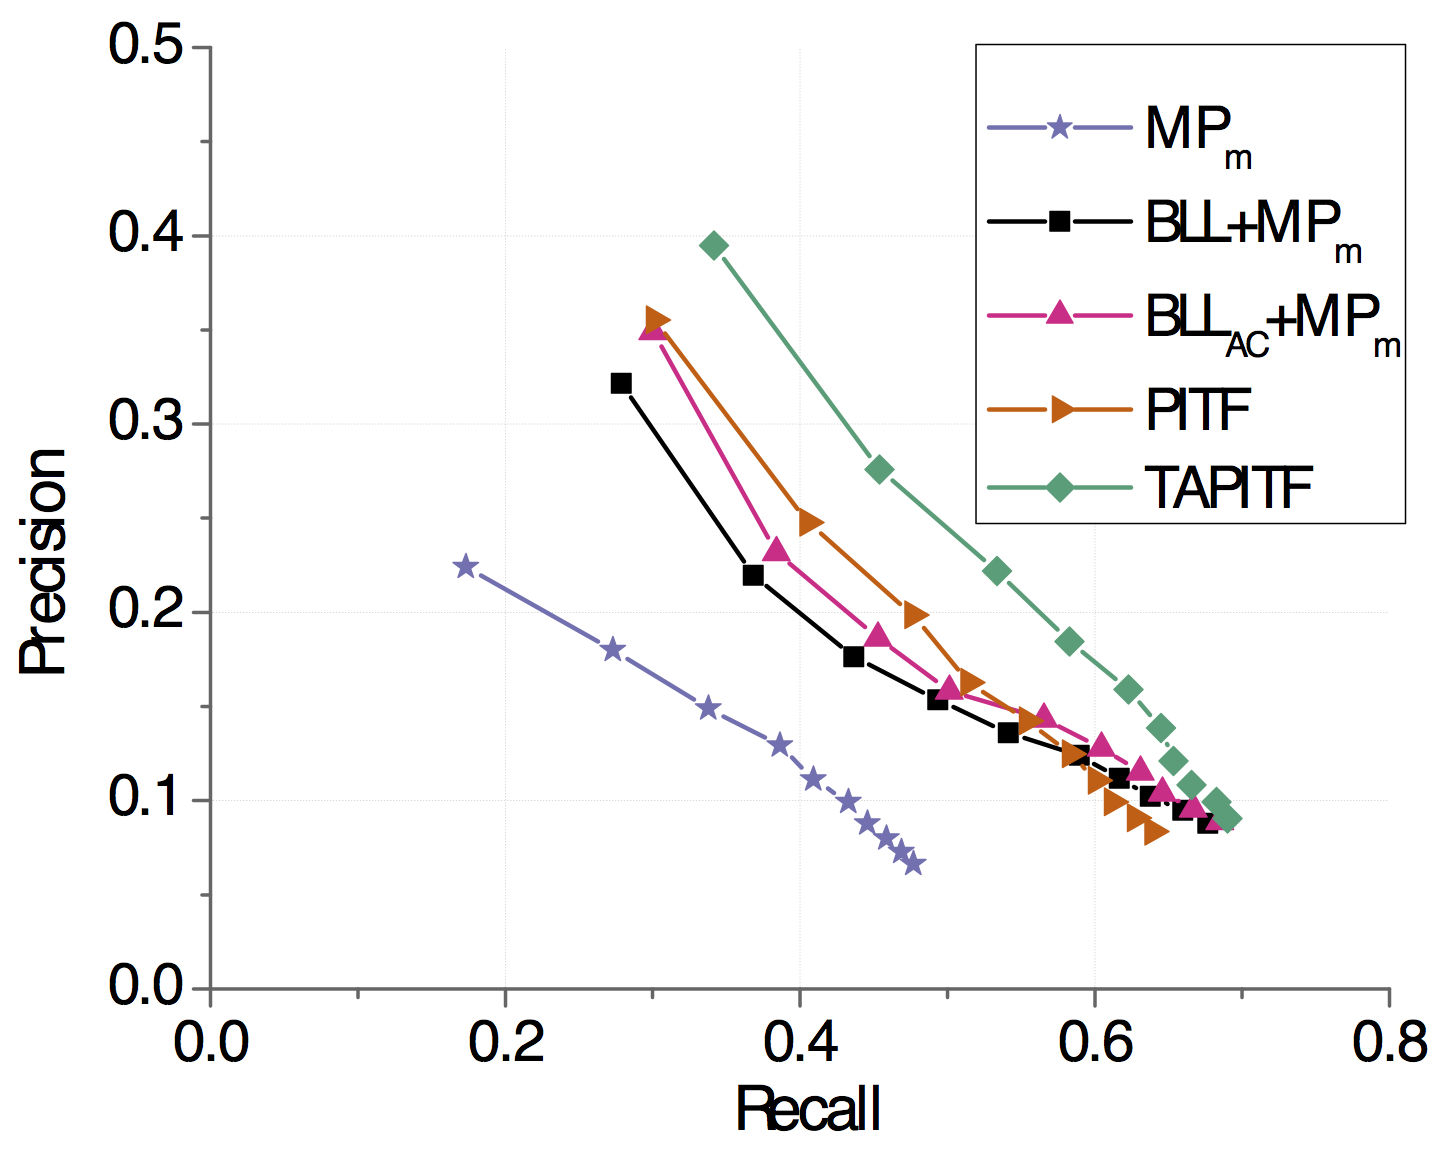
\includegraphics[width=0.485\textwidth]{Fig/wpitf/prm3}}
	\subfigure[LastFM (no core)]{
		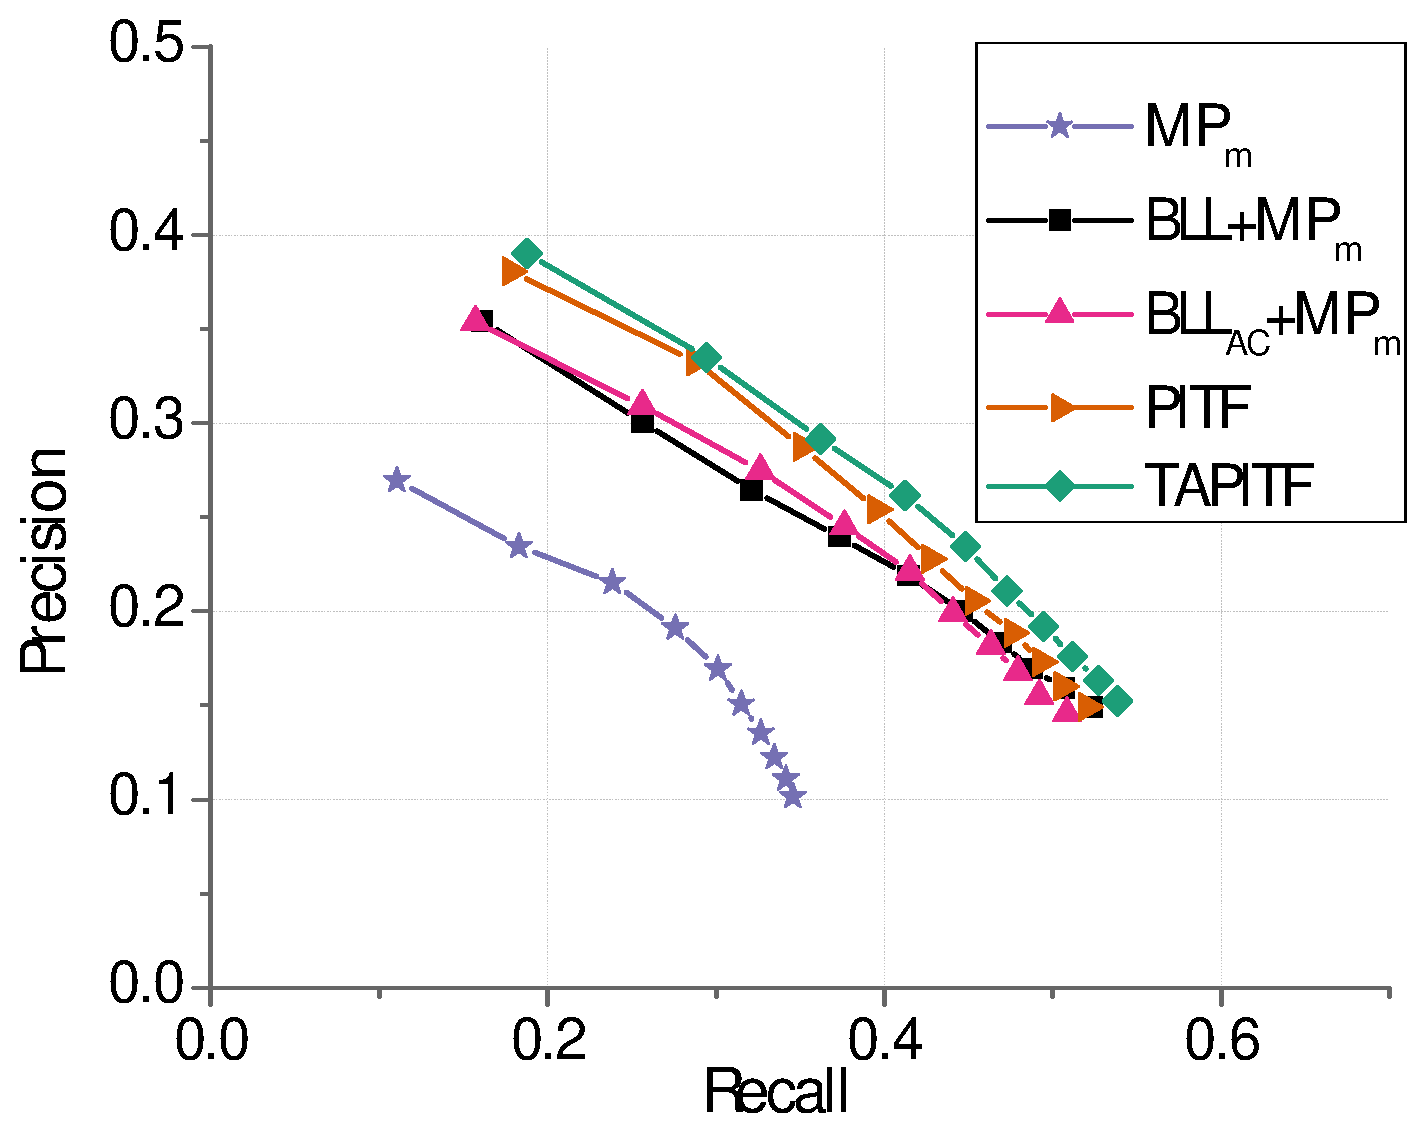
\includegraphics[width=0.485\textwidth]{Fig/wpitf/prl1}}
	\hspace{0.0cm}
	\subfigure[LastFM (core 3)]{
		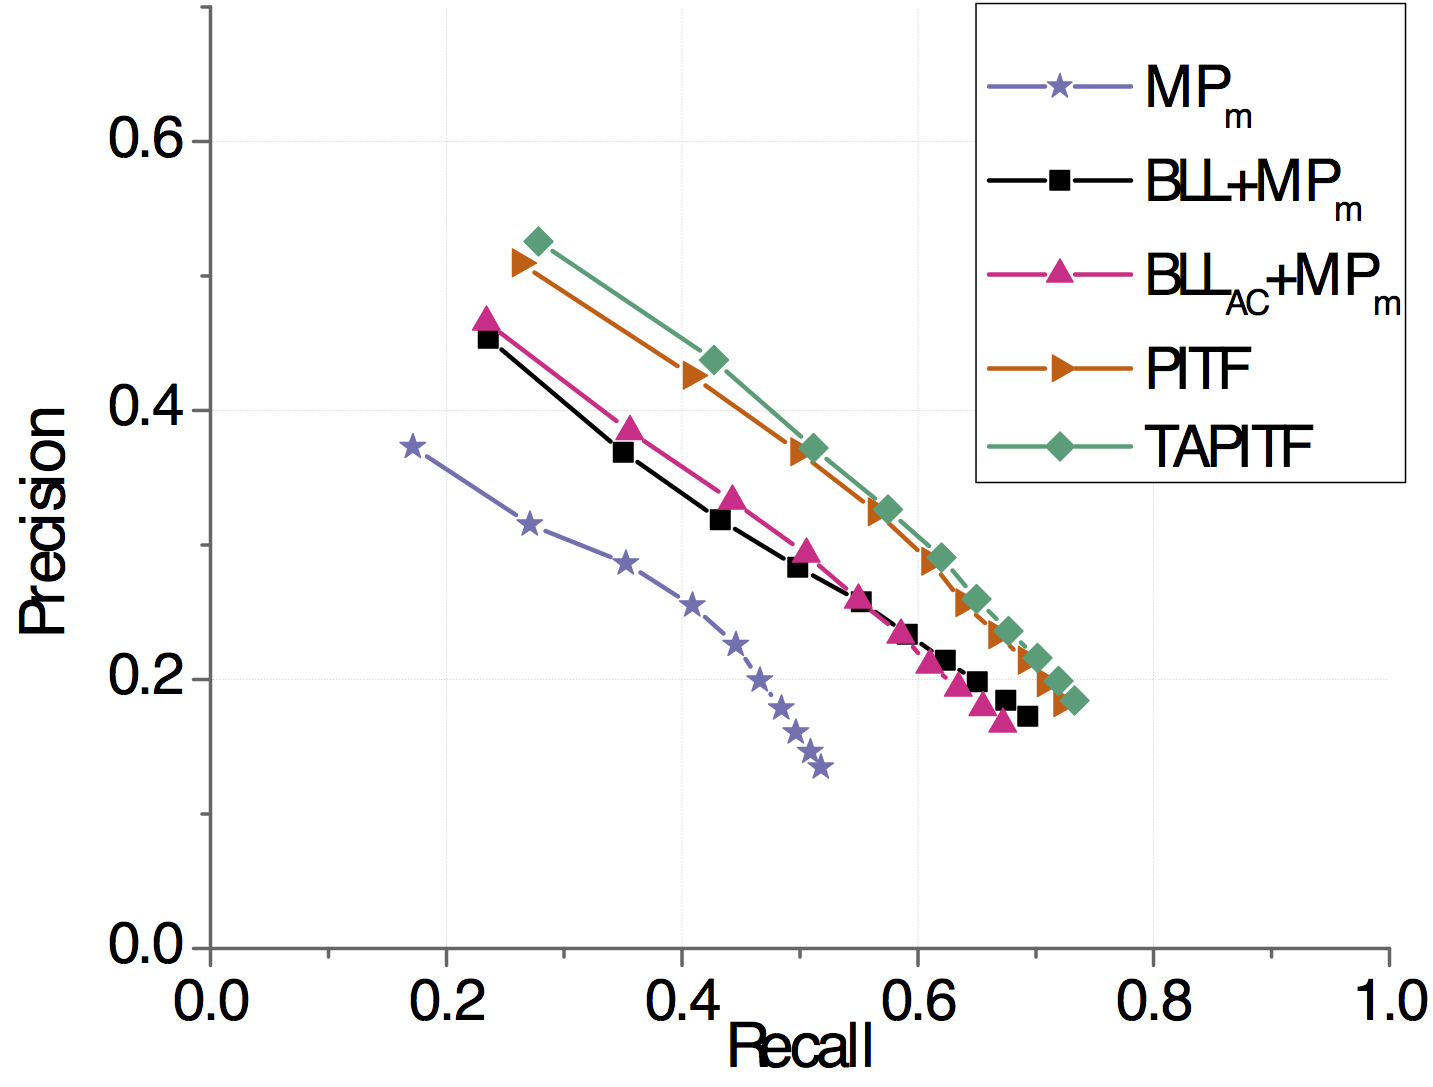
\includegraphics[width=0.485\textwidth]{Fig/wpitf/prl3}}
	\subfigure[Delicious (no core)]{
		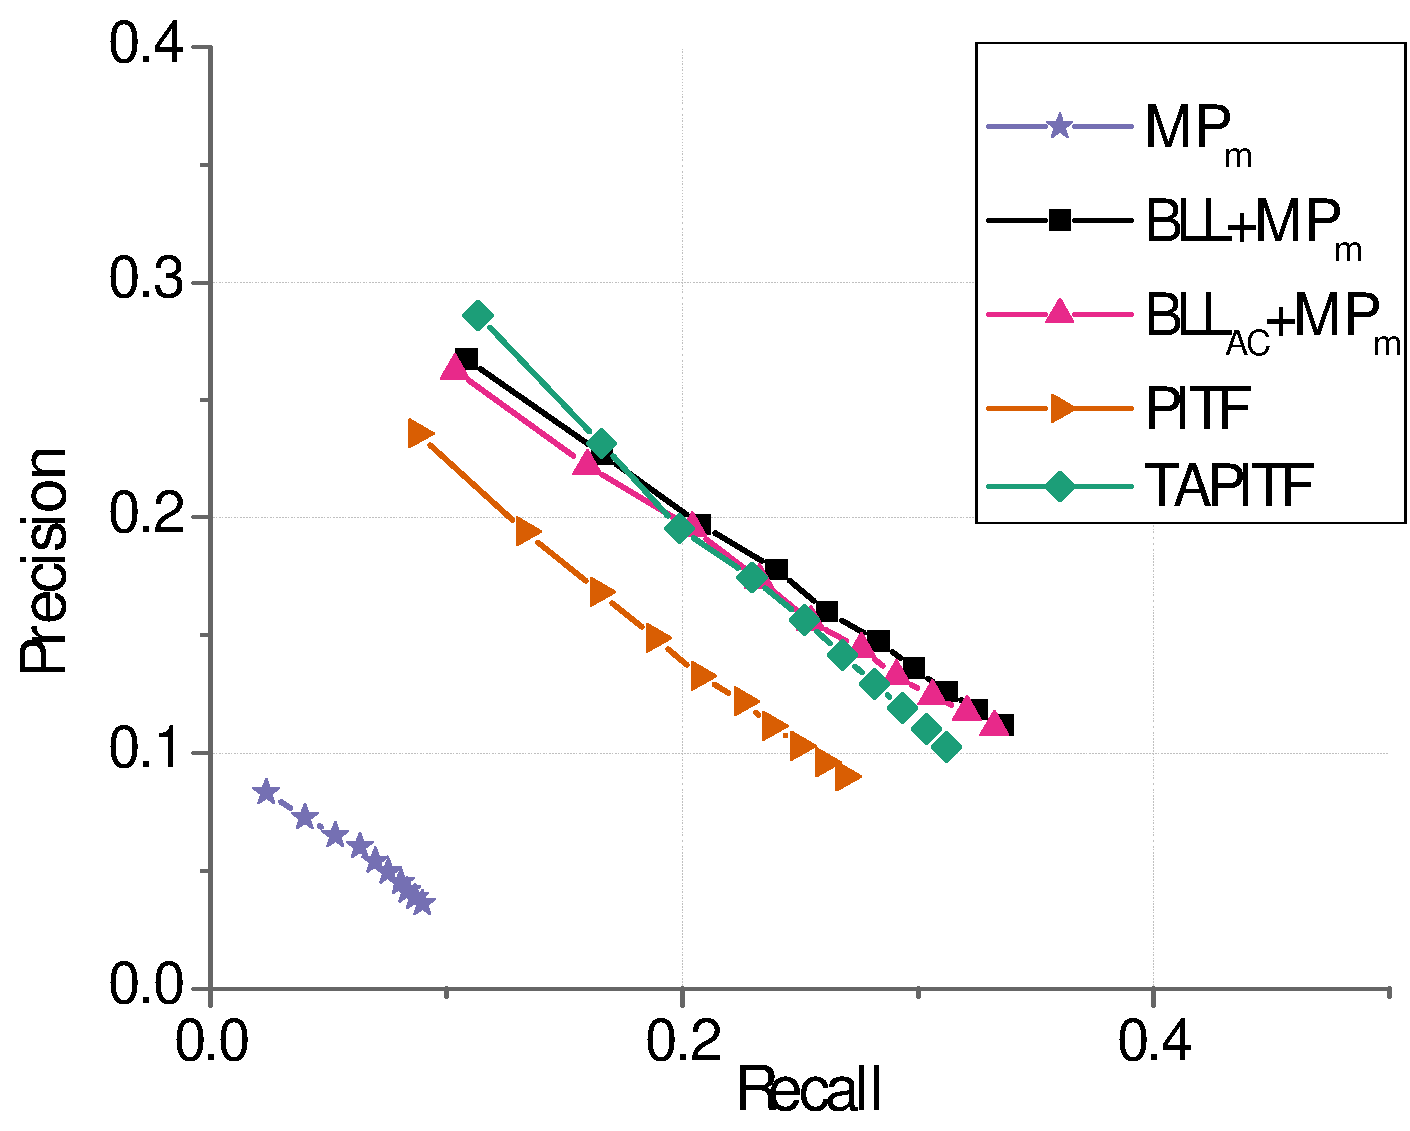
\includegraphics[width=0.485\textwidth]{Fig/wpitf/prd1}}
	\hspace{0.0cm}
	\subfigure[Delicious (core 3)]{
		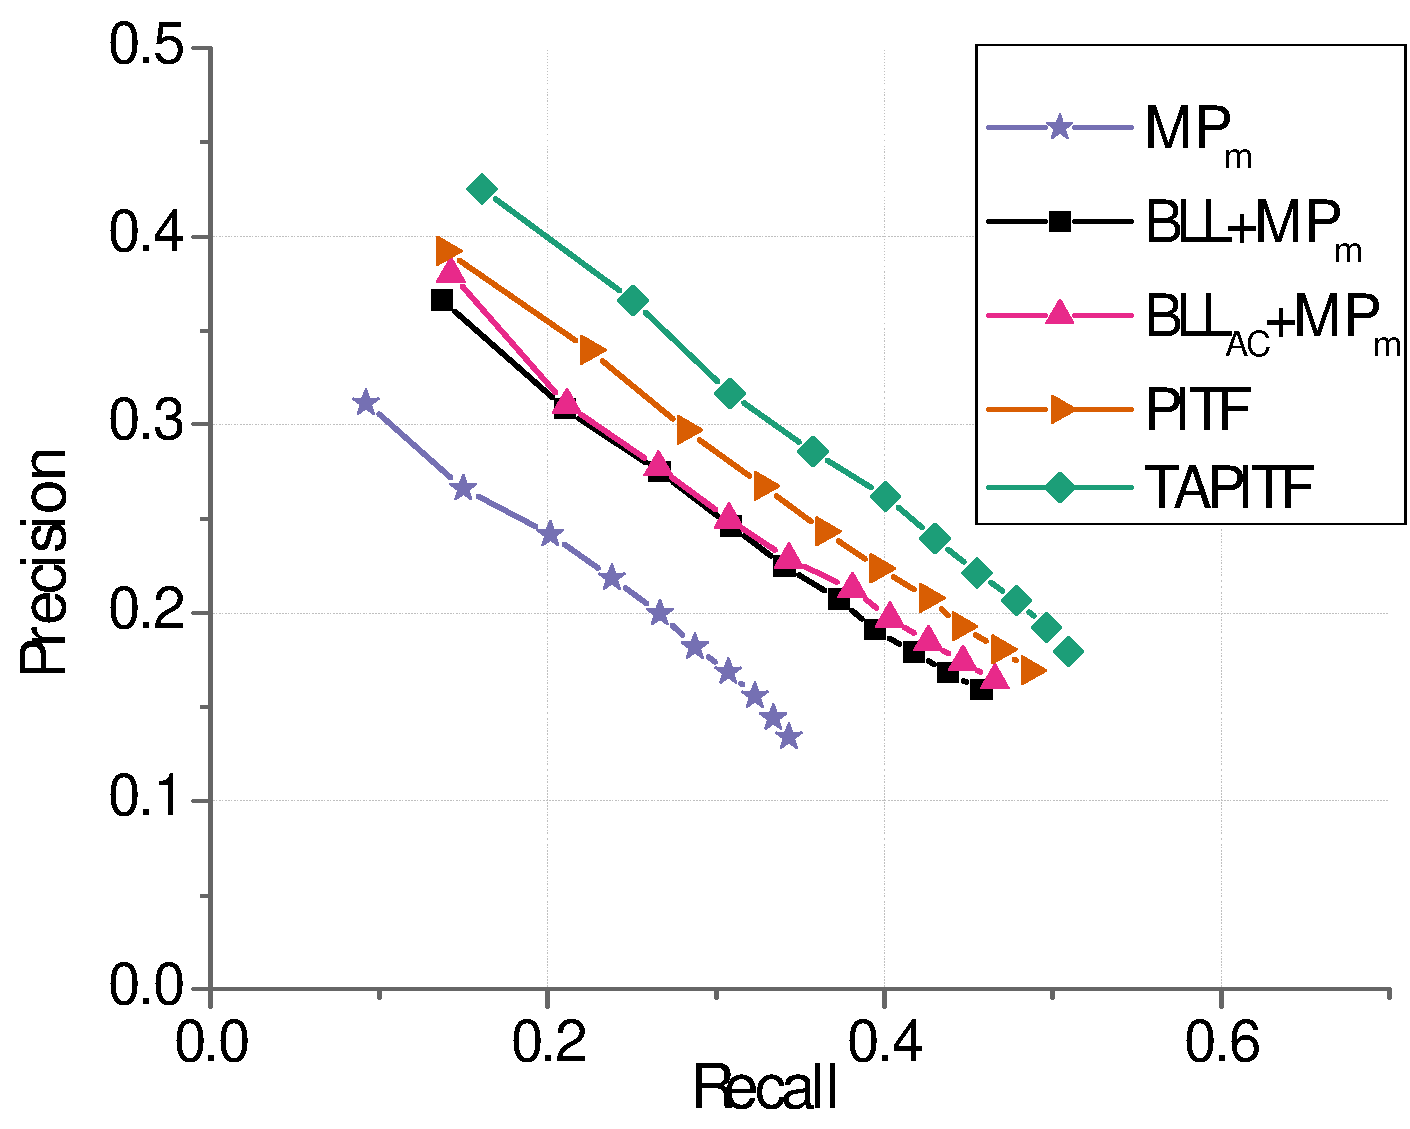
\includegraphics[width=0.485\textwidth]{Fig/wpitf/prd3}}
	\caption{各类标签推荐模型的召回率/精准率曲线}
	\label{fig-wpitf-pr}
\end{figure}

\subsubsection{权重因子 对 TAPITF 推荐结果的影响}
本小节中实验设置用户-标签-时间与商品-标签的权重因子相同,通过改变$\alpha$来观察 TAPITF 的性能 变化 (F1@5)。从图\ref{fig-wpitf-alpha}可以看出来,对所有的数据集, 随着$\alpha$值的增大,TAPITF 的性能不断提高,直到达 到最优值,继续增大$\alpha$,TAPITF 的性能会逐渐下降 (对数据集 LastFM core 3 的情况,如果将$\alpha$值调成负 数,那么 TAPITF 性能会明显下降,所以其最优值 就是在$\alpha=0$时取得)。当权重值$\alpha$调到最优时,可看
到TAPITF在所有数据集上基本都是优于 PITF 和 BLL+MP$_m$(最差也能与这两种方法持平),这说明通过 对 PITF 的用户-标签-时间与商品-标签上增加合理的 权重可以有效改善推荐性能。并且在对数据集过 滤之后 (core 3),可以看到 TAPITF 的性能明显优于其他对比方法。这有可能因为 PITF 对较稠密数据有 着更好的推荐效果,所以明显优于 BLL+MP$_m$,而本章提出的TAPITF方法在 PITF 的基础上考虑了时间对用 户行为的影响,性能得到进一步的提升。同时,实验结果中可以发现基于时间信息建模的标签推荐方法在冷启动方面要优于原始张量分解模型,体现这类方法在数据稀疏时的优势。

在接下来的实验中选择 TAPITF性能最好时的$\alpha$值来与其他模型的实验结果做对比,对数据集 Movielens core 3 取$\alpha=1.2$,对数据集 LastFM core 3 取$\alpha=0$,其他情况下均取$\alpha=0.8$。

\subsubsection{与其他标签推荐方法对比分析}

本小节实验将本章节提出的TAPITF模型与当前最新的一些标签推荐方法进行对比。图\ref{fig-wpitf-pr}显示在数据集 Movielens、LastFM 和 Delicious 上,TAPITF与其他标签推荐方法在TOP 1 到 TOP 10 上的召回率/精准率曲线。从总体上来说,对于所有数据集TAPITF基本上都是性能最优的,这进一步说明了在PITF中加 入时间对用户行为的影响是十分有效的。在未过滤的 数据集 Movielens 和 Delicous 上,尽管当推荐的 TOP n列表长度较大时,TAPITF性能略差于BLL+MP$_m$ 和 BLL$_{AC}$+MP$_m$,但是在实际应用中,对于一个给定的商品,用户关注的标签往往不会太多,有时甚至只会 关心排名最前的那个标签。所以在这种情况下,依然可以认为TAPITF方法是有效的。

在新颖性上,从表~\ref{tab-wpitf-aip}可以看出,PITF在所有数据集上的新颖性都是最好的,而TAPITF 的新颖性 略次于 PITF,但是优于 MP$_m$,BLL+MP$_m$ 和 BLL$_{AC}$+MP$_m$。 这说明TAPITF模型在获得最优准确度的前提下,还能得到较好的新颖度。而BLL类方法完全基于用户和商品的历史标签,导致新颖度非常低,这其实不利于推荐系统的发展。
\begin{table}
	\centering
	\caption{不同方法的AIP@10结果对比}
	\label{tab-wpitf-aip}%
	\begin{tabular}{|c||c|c|c|c|c|c|}
		\hline
		DataSet  & Core  & MP$_m$   & BLL+MP$_m$ & BLL$_{AC}$+MP$_m$ & PITF  & TAPITF \bigstrut \\
		\hline
		\hline
		\multirow{2}[4]{*}{Movielens } & -     & 0.806  & 0.788  & 0.786  & \textbf{0.854 } & 0.812  \bigstrut\\
		\cline{2-7}          & 3     & 0.761  & 0.762  & 0.757  & \textbf{0.803 } & 0.777  \bigstrut\\
		\hline
		\multirow{2}[4]{*}{LastFM } & -     & 0.732  & 0.724  & 0.709  & \textbf{0.779 } & 0.764 \bigstrut \\
		\cline{2-7}          & 3     & 0.668  & 0.660  & 0.639  & \textbf{0.697 } & \textbf{0.697 } \bigstrut\\
		\hline
		\multirow{2}[4]{*}{Delicious } & -     & 0.881  & 0.873  & 0.878  & \textbf{0.949 } & 0.912 \bigstrut \\
		\cline{2-7}          & 3     & 0.787  & 0.767  & 0.767  & \textbf{0.827 } & 0.778 \bigstrut \\
		\hline
	\end{tabular}%
	
\end{table}%
\subsubsection{TAPITF 对比 PITF}

图\ref{fig-wpitf-number}显示了 TAPITF 和 PITF 在不同迭代次数下
的准确度对比,为了确保算法达到收敛,本小节实验设置迭代轮数为100轮。从图中可以明显的看出,本章节提出的TAPITF 模型在数据集 Movielens、LastFM 以及 Delicious no core 和 core 3 上的准确度和收敛速度都要优于 PITF。TAPITF 在所有数据集上都能在40轮迭代前收敛,而PITF基本上要达到60轮迭代之后才逐渐收敛,而且 TAPITF在前20轮的收敛速度要远快于PITF,主要原因是加入了用户-标签-时间权重和商品-标签权重。因此即使不进行参数学习,TAPITF也可以拥有类似于BLL类模型的推荐效果。

而在运行时间上,相比 PITF,TAPITF由于在每轮迭代过程中要额外计算用户-标签-时间的权重因 子,所以每轮迭代的时间要比PITF慢。表 \ref{tab-wpitf-effiency}显示了 TAPITF与PITF在不同数据集上运行时间对比,本节实验选取了 100 轮迭代时间的平均值作为最终运行时 间(其中每轮迭代为训练集样本数目的 100 倍)。可以看出TAPITF在数据集 LastFM 和 Delicious 上的运行时间比PITF略长,而在数据集上Movielens上时间要比PITF长很多。但是如章节\ref{subsec-wpitf-timeAnalysis}所示,经过计算统计,因为在数据集 Movielens 上的期望值要比另外两个数据集大 10 倍以上,也就 是说 Movielens 的数据十分稠密,所以 TPWPITF 的 运行时间要比 PITF 长很多,而在当前互联网时代,数据往往都是非常稀疏的,所以在大多数情况下,本章模型仍然是十分有效的。

\begin{figure}
	\centering
	\subfigure[Movielens (no core)]{
		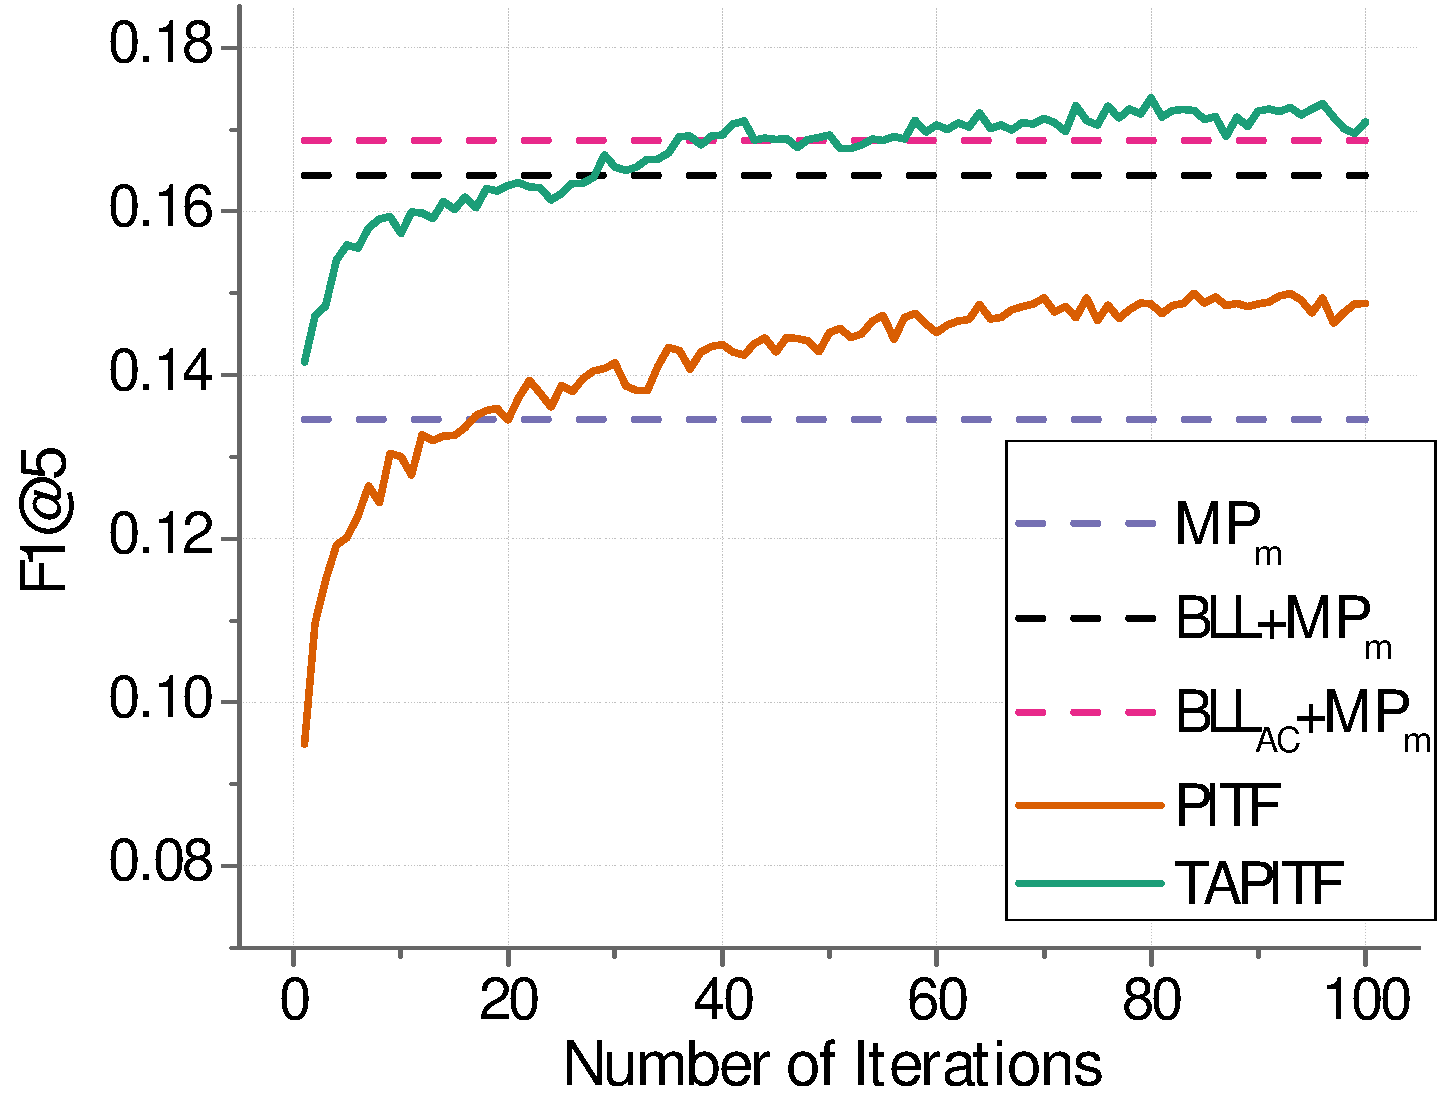
\includegraphics[width=0.45\textwidth]{Fig/wpitf/numberm1}}
	\hspace{0.8cm}
	\subfigure[Movielens (core 3)]{
		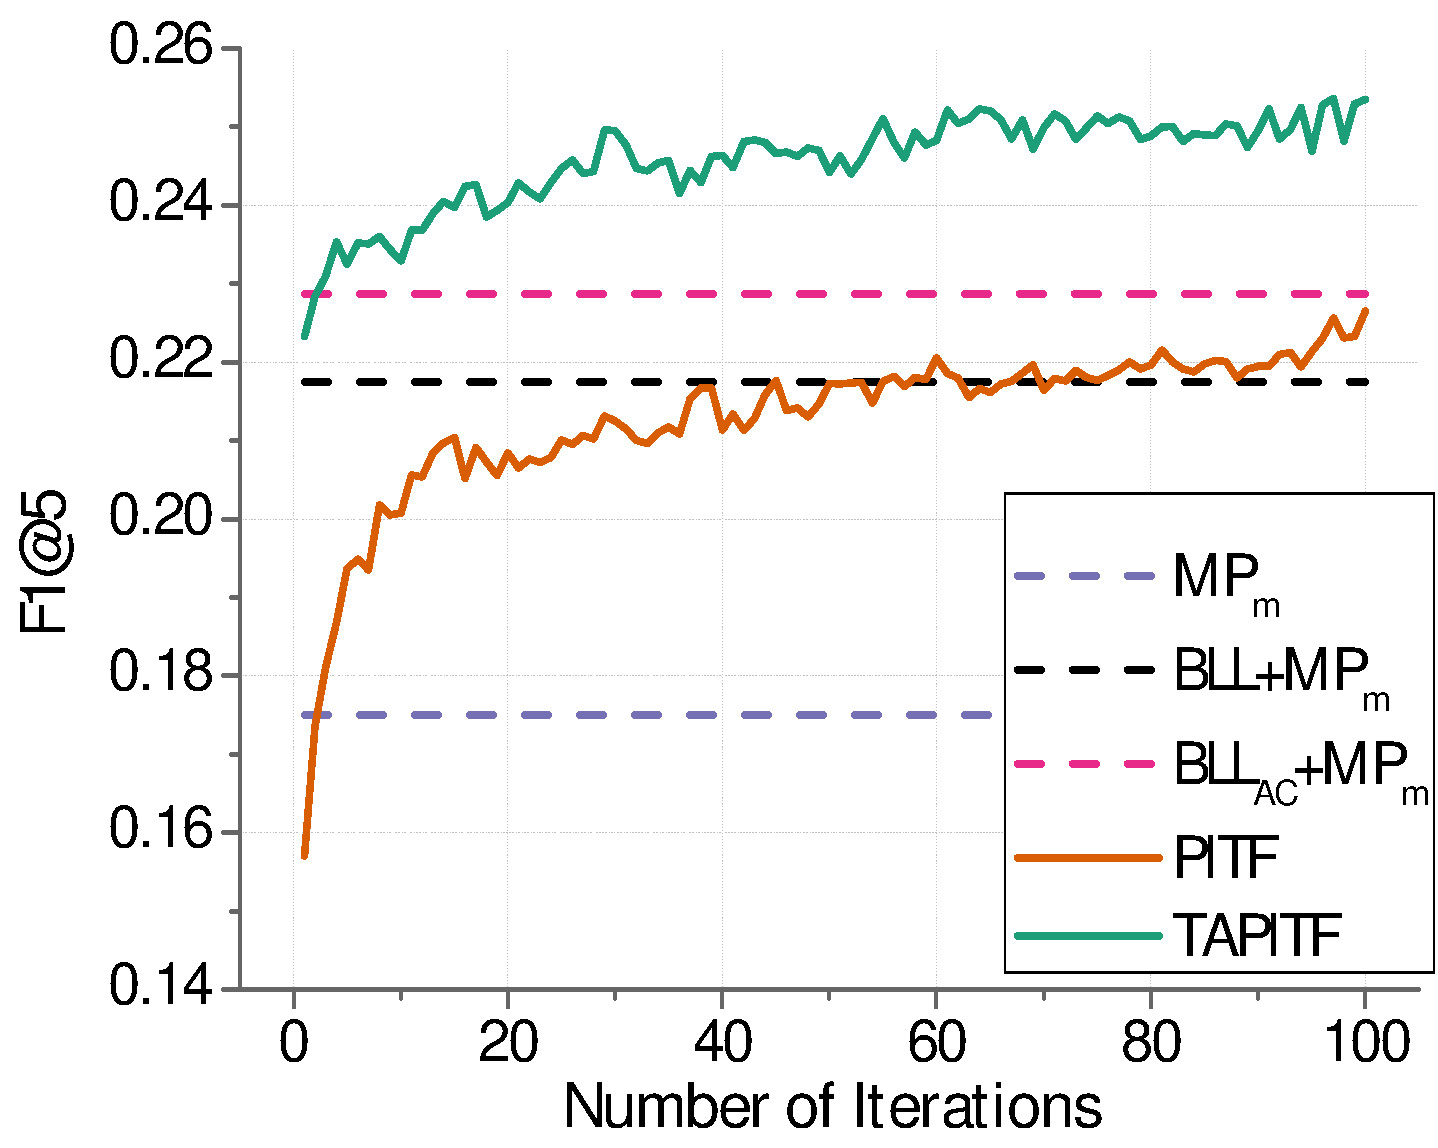
\includegraphics[width=0.45\textwidth]{Fig/wpitf/numberm3}}
	\subfigure[LastFM (no core)]{
		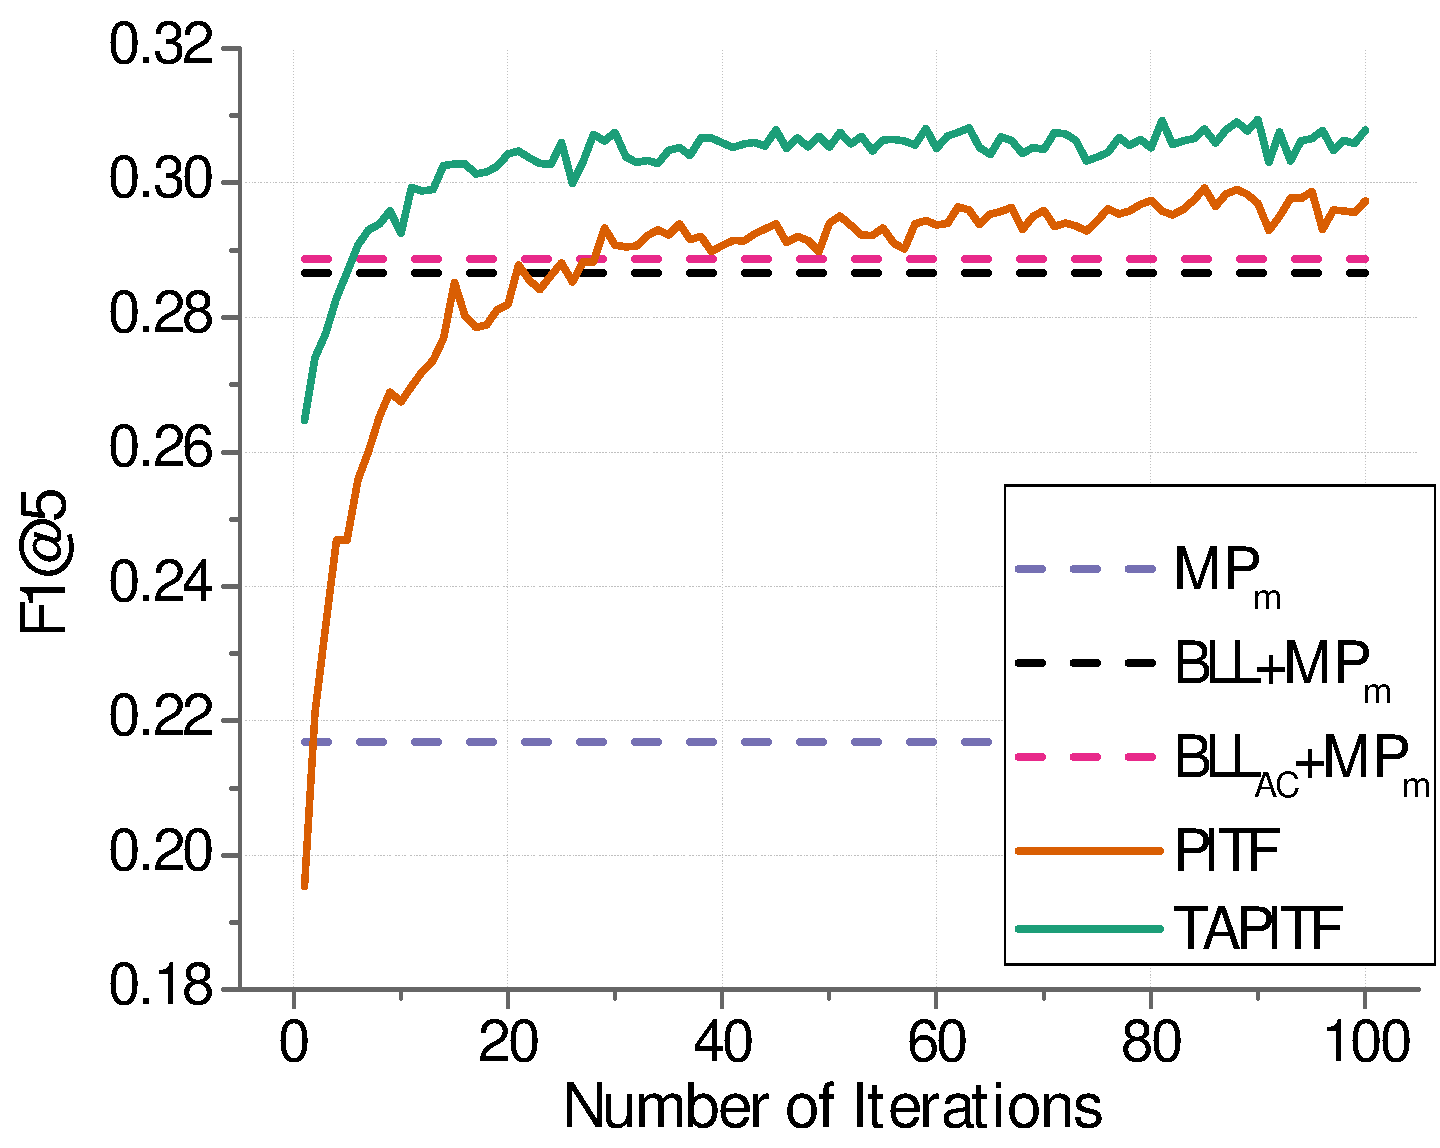
\includegraphics[width=0.45\textwidth]{Fig/wpitf/numberl1}}
	\hspace{0.8cm}
	\subfigure[LastFM (core 3)]{
		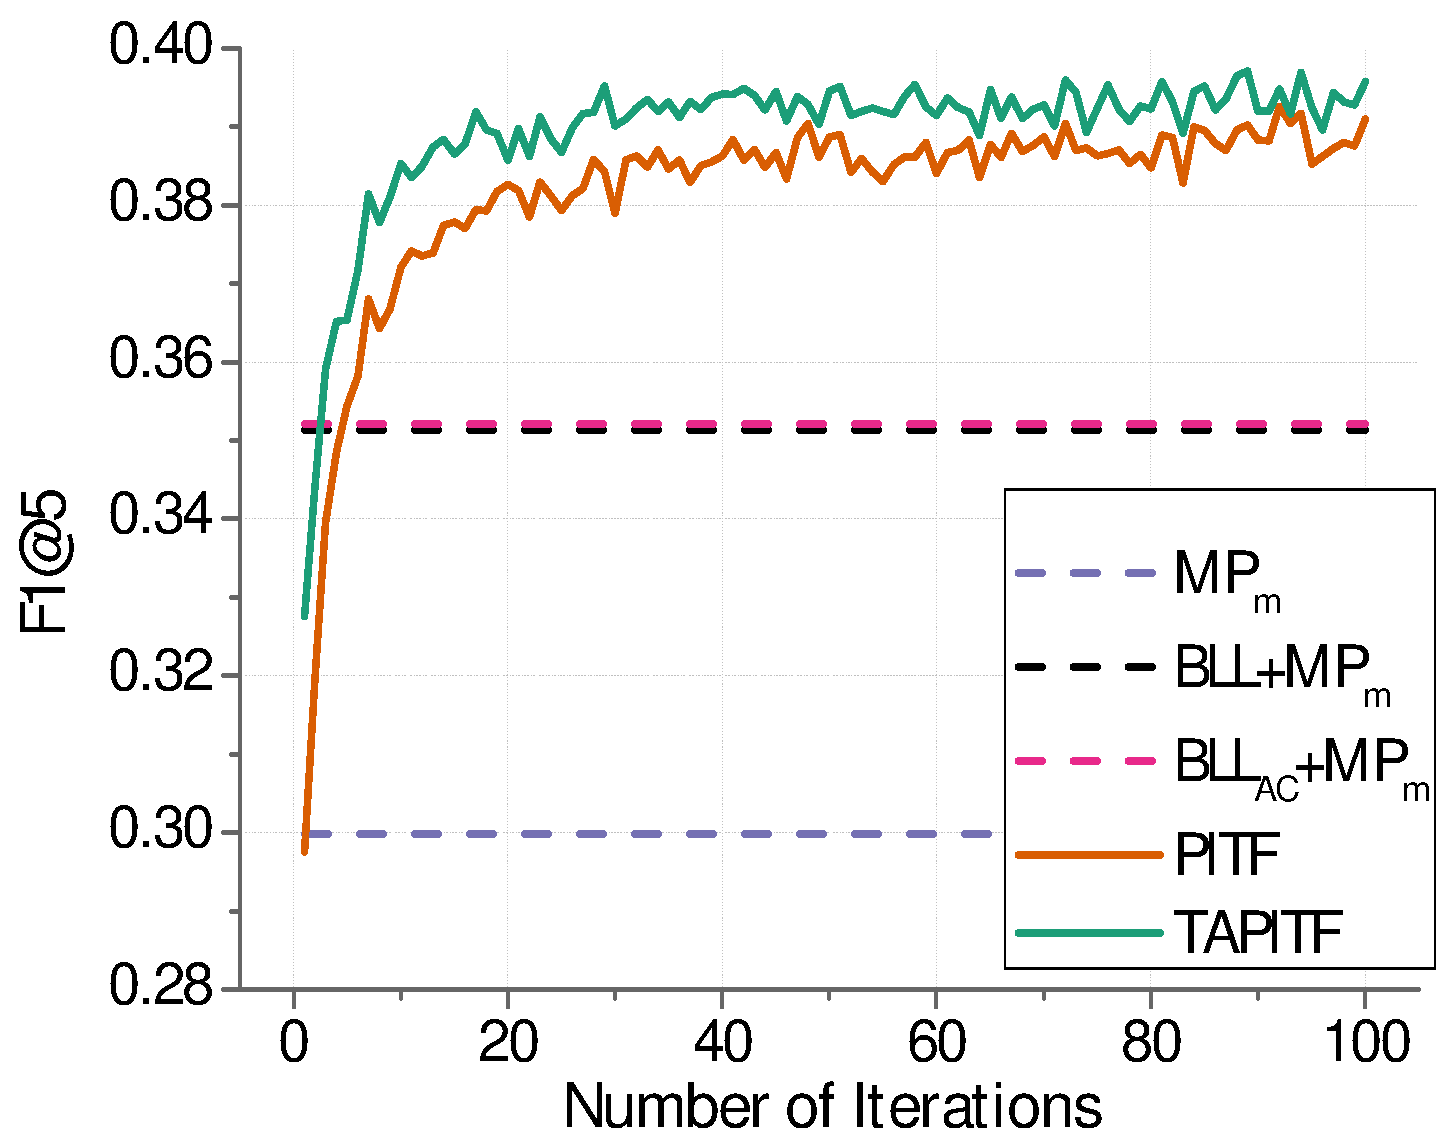
\includegraphics[width=0.45\textwidth]{Fig/wpitf/numberl3}}
	\subfigure[Delicious (no core)]{
		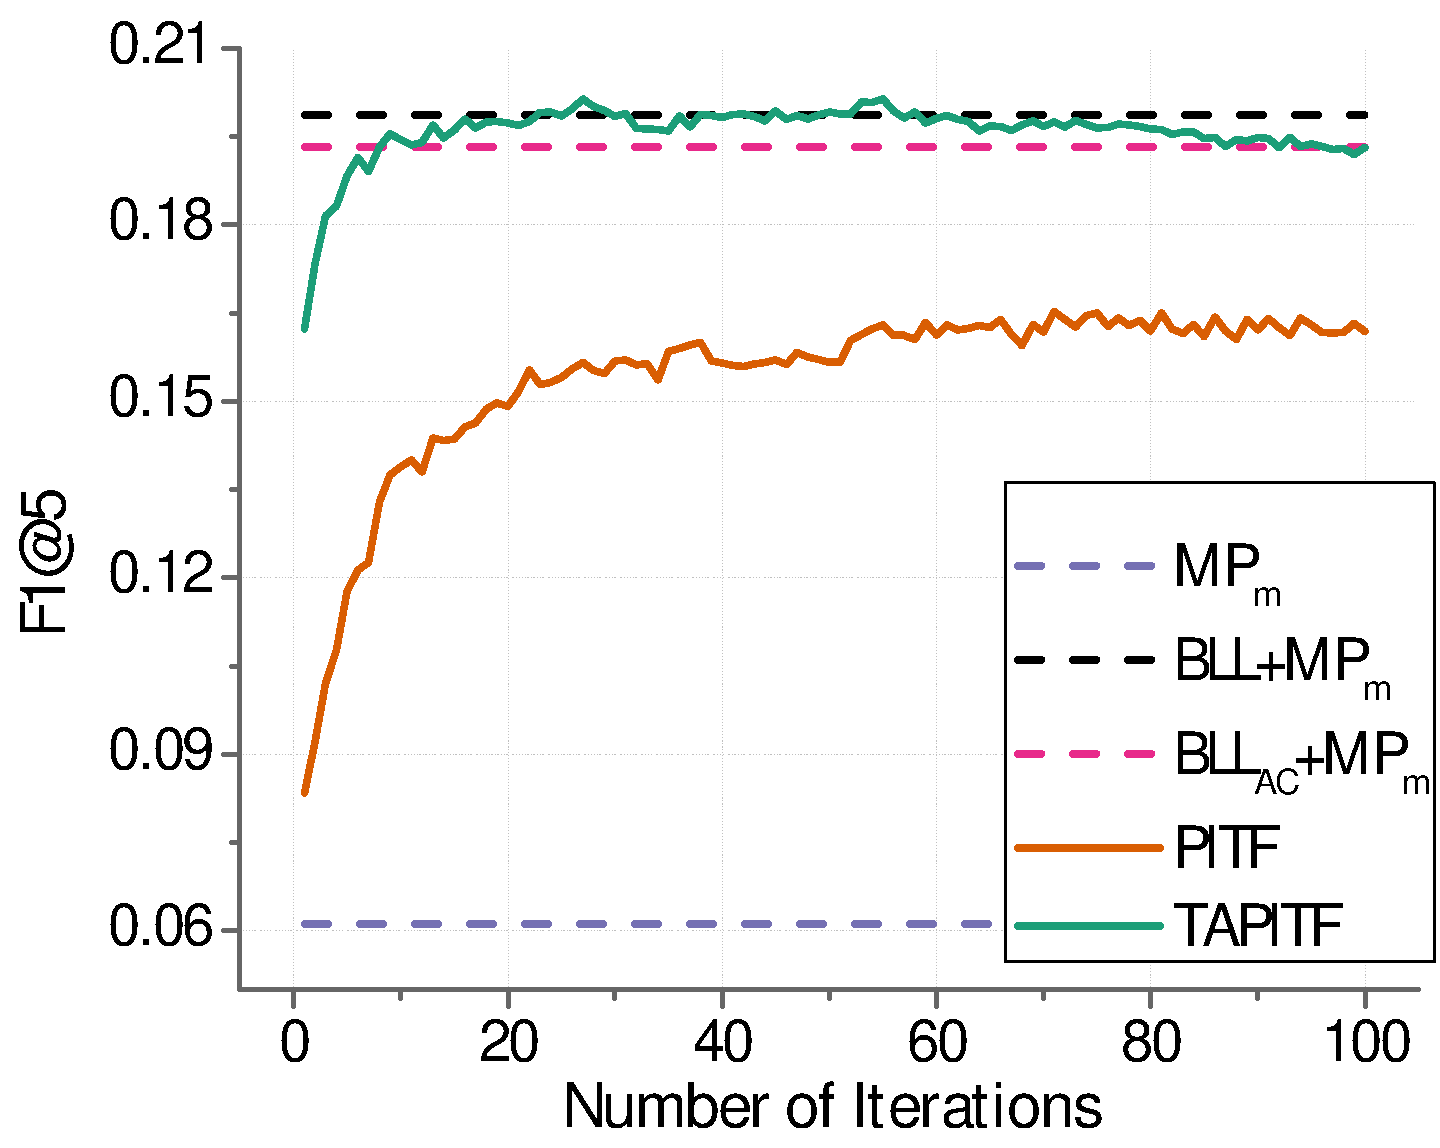
\includegraphics[width=0.45\textwidth]{Fig/wpitf/numberd1}}
	\hspace{0.8cm}
	\subfigure[Delicious (core 3)]{
		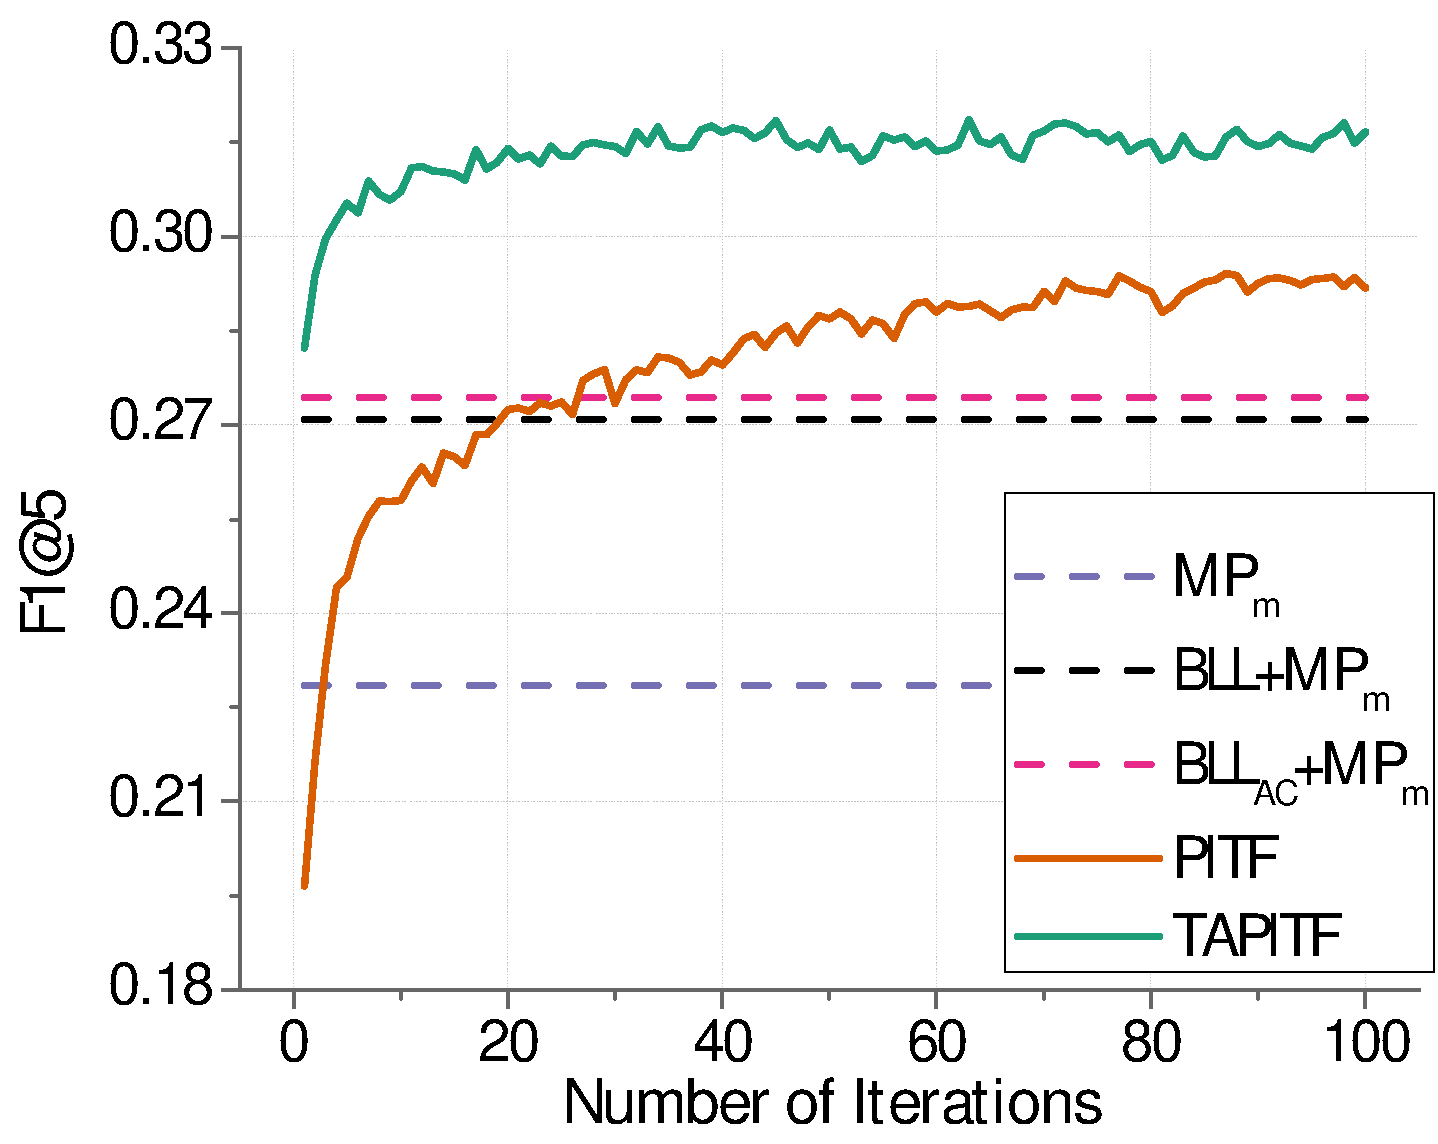
\includegraphics[width=0.45\textwidth]{Fig/wpitf/numberd3}}
	\caption{TAPITF 和 PITF的准确率与收敛速度对比}
	\label{fig-wpitf-number}
\end{figure}

\begin{table}
  \centering
  \caption{TAPITF 与 PITF的参数学习时间对比}
  	 \label{tab-wpitf-effiency}
    \begin{tabular}{|c||c|c|c|}
    \hline
    DataSet  & Core  & PITF  & TAPITF \bigstrut\\
    \hline
    \hline
    \multirow{2}[4]{*}{Movielens } & -     & 10.3  & 31.3  \bigstrut\\
\cline{2-4}          & 3     & 5.8   & 23.2  \bigstrut\\
    \hline
    \multirow{2}[4]{*}{LastFM } & -     & 41.4  & 51.7  \bigstrut\\
\cline{2-4}          & 3     & 32.6  & 44.6  \bigstrut\\
    \hline
    \multirow{2}[4]{*}{Delicious } & -     & 110.7  & 145.0  \bigstrut\\
\cline{2-4}          & 3     & 16.8  & 24.0  \bigstrut\\
    \hline
    \end{tabular}%

\end{table}%


\section{本章小结}
\label{sec-wpitf-conclusion}
本章节综合分析现阶段个性化标签推荐系统的优缺点,提出了时间感知的张量分解模型TAPITF。本章节工作从时间点过程对时间信息建模角度出发,利用指数函数将Hawkes过程从叠加转化为递归形式,使得计算用户当前时间对标签的喜好值只跟上次使用标签的时间有关,极大地减少了计算时间。然后,本章节工作将用户-标签-时间关系信息以及商品-标签关系信息以权重的方式与PITF模型结合,使得本章模型既能考虑用户标注标签行为随时间变化而变化的现象,也能有效地利用相似用户、相似商品、相似标签的信息,从而更好地对用户对商品标注标签的行为进行建模,提高标签推荐的准确度和新颖性。通过在不同场景的真实数据上进行实验,表明TAPITF在准 确性上优于当前流行的个性化标签推荐算法,同时有较好的推荐新颖性。

\clearpage
\phantom{s}
\clearpage